\chapter{The UK Light Injection System}
\epigraph{``Photon torpedo: isn't that the universal greeting when communications are down?''\newline
``I think it's the universal greeting when you don't like someone.''}{William T. Riker and Geordi La Forge \newline Star Trek: Insurrection (1998)}
\label{chp:ukli}

The UK calibration group's efforts have been focussed on improving the data analysis method and improving the accuracy of the water coefficient measurements. To aid this effort a new UK developed Light Injection (UKLI) system was installed into Super-Kamiokande during the refurbishment that ocurred in the summer of 2018. This system has its own set of optics with multiple beam spot diameters and will be described in detail in this Chapter. 

\section{The UK Light Injection System Electronics and Optics}

The electronics setup architecture for the UK Light Injection System is made of sixteen light emitting diode boards, where the light being pulsed by the LEDs has a wavelength of 435 nm and there is 1 LED per injector. Each LED is coupled to three optical fibres: one channel connected to a monitor PMT, one connected to an optical fibre that sends light into the Super-Kamiokande detector, and one is a spare.
\newline

Unlike the Korean laser system mentioned in Chapter 4 which injects light into the detector using an optical fibre which has an opening angle of 12 degrees, the UK Light Injection system contains three different types of light injection optics, with each having a different opening angle: a bare fibre, a collimator and a diffuser. This range of optics can accomadate a larger variety of calibration measurements, and better suit the multiple applications of the light injection system. 

\subsubsection{The Collimator Optic}

A 2-degree opening half angle is achieved by the collimator optic by using a GRIN (gradient-index) lens \cite{grin_lens} to reduce the opening angle of the light coming from the fibre optic. A schematic of the collimator design can be seen in Figure \ref{fig:collimator_schematic}. 

\begin{figure}
    \centering
    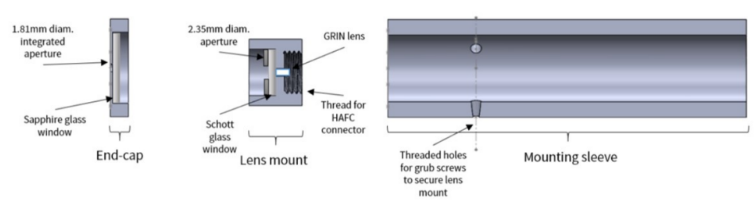
\includegraphics[width=0.8\textwidth]{Figures/collimator_schematic.png}
    \caption{Collimator schematic including the end-cap, lens mount and mounting sleeve structures.}
    \label{fig:collimator_schematic}
\end{figure}


\subsubsection{The Diffuser Optic}

The diffuser optic is a wide angled beam with an opening half-angle of 40 degrees, allowing for more PMT coverage in the detector, therefore enabling measurements of PMT properties, and measurements of light attenuation length in water. Figure \ref{fig:diffuser_photo} shows a photograph of one of the diffusers used, and one of the diffuser ball enclosures. The enclosure is made of high grade stainless steel and using a chemical and water resistant epoxy resin, so all the components were ensured to be watertight. 

\begin{figure}
    \centering
    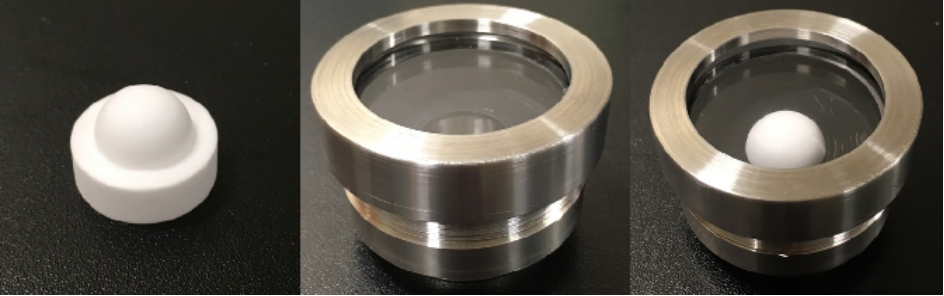
\includegraphics[width=0.7\textwidth]{Figures/diffuser_photo.png}
    \caption{Photograph of the diffuser by itself (left), empty diffuser enclosure (centre) and diffuser inside enclosure (right).}
    \label{fig:diffuser_photo}
\end{figure} 

\subsubsection{Bare Fibre and Optical Plate}

The bare fibre injector are 1 mm step index fibres, are approximately 20 cm in length and are used for validation purposes with the bare fibres in the Korean optical calibration system. These short fibres are screwed into the back end of the optical plate that the collimator and diffuser optics are mounted on, shown in Figure \ref{fig:optical_plate}.

\begin{figure}
    \centering
    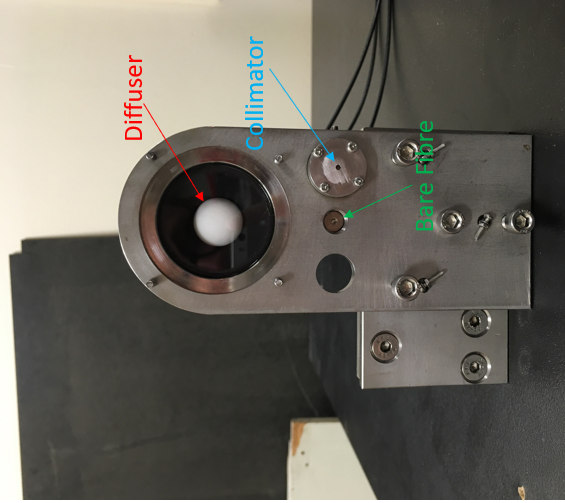
\includegraphics[width=0.7\textwidth, angle =270]{Figures/optical_plate.png}
    \caption{Photograph of the optical plate which houses the different optics.}
    \label{fig:optical_plate}
\end{figure}


\section{Optics test stand measurements}

In order to test the collimator and diffuser optics, measurements of the angular distributions were made using diffuser and collimator test-stands and would measure angular distributions of the light intensity. The setup for the collimator test stand at the University of Warwick is shown in Figure \ref{fig:coll_test_stand} and captures the beam cross section by moving a CMOS camera along the beam width. For the diffuser test-stand the angular distribution of the light output was measured using the setup shown in Figure \ref{fig:diffuser_test_stand}. This test stand setup for the diffuser optics consists of a test diffuser ball placed inside a diffuser enclosure, a rotation stage which allows for the movement of the diffuser between -40 and 40 degrees, and a PMT used for pulse intensity measurement set up 250 mm away from the diffuser. An optical fibre couples the diffuser under test to a laser set to a wavelength of 450 nm. 

\begin{figure}
    \centering
    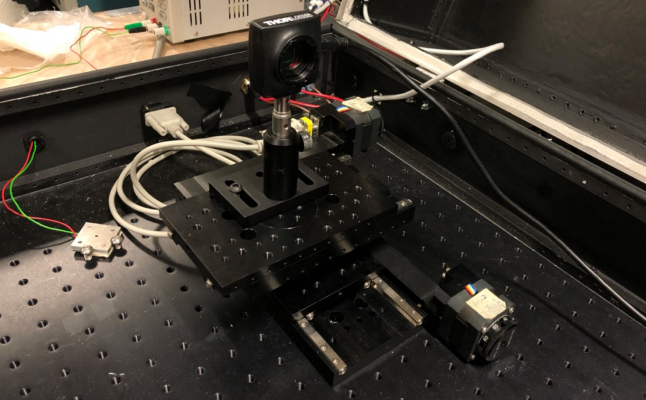
\includegraphics[width=0.7\textwidth]{Figures/coll_test_stand.png}
    \caption{Setup of the collimator test stand provided by the University of Warwick.}
    \label{fig:coll_test_stand}
\end{figure}

Figure \ref{fig:collimator_TF1} shows fits made by ROOT to the light profiles for the collimator. The angular distributions shown give the distribution of the polar angle in degrees of light intensity which are relative to the virtual position from which the light cone originates, averaged over all the orientations of the azimuthal angle. 

\begin{figure}[!htbp]
    \centering
    
    
    
    \subfloat[]{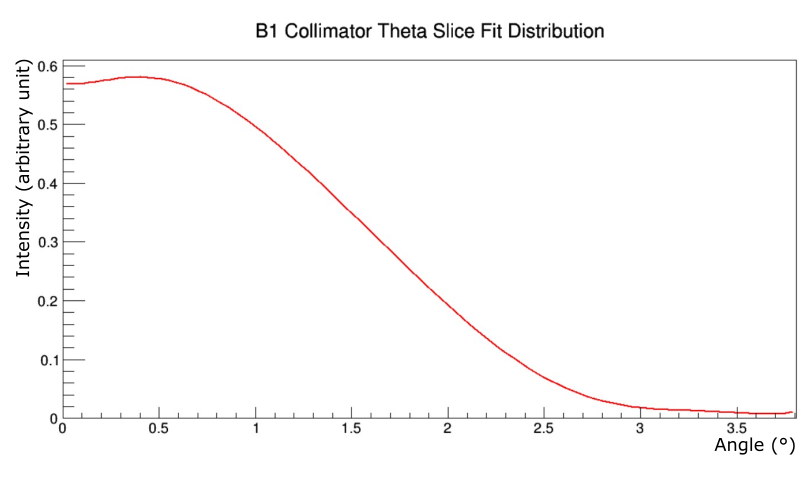
\includegraphics[width=0.49\textwidth]{Figures/B1_collimator_fit.PNG}}\hfill
    \subfloat[]{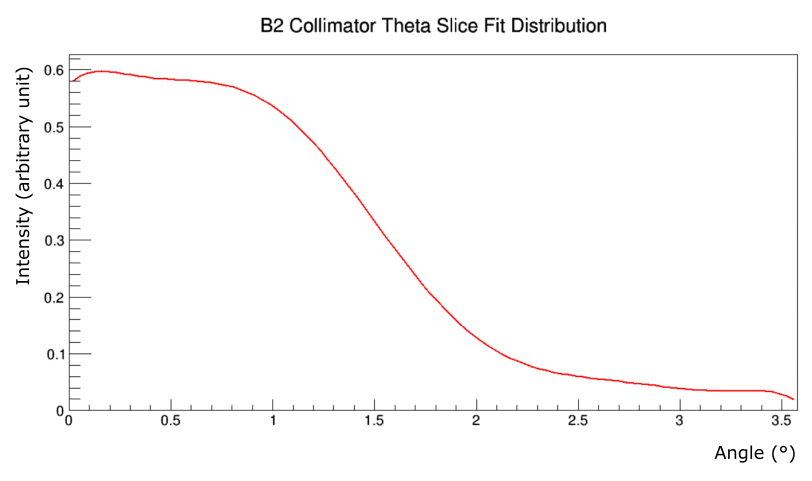
\includegraphics[width=0.49\textwidth]{Figures/B2_collimator_fit.PNG}}\par
    \subfloat[]{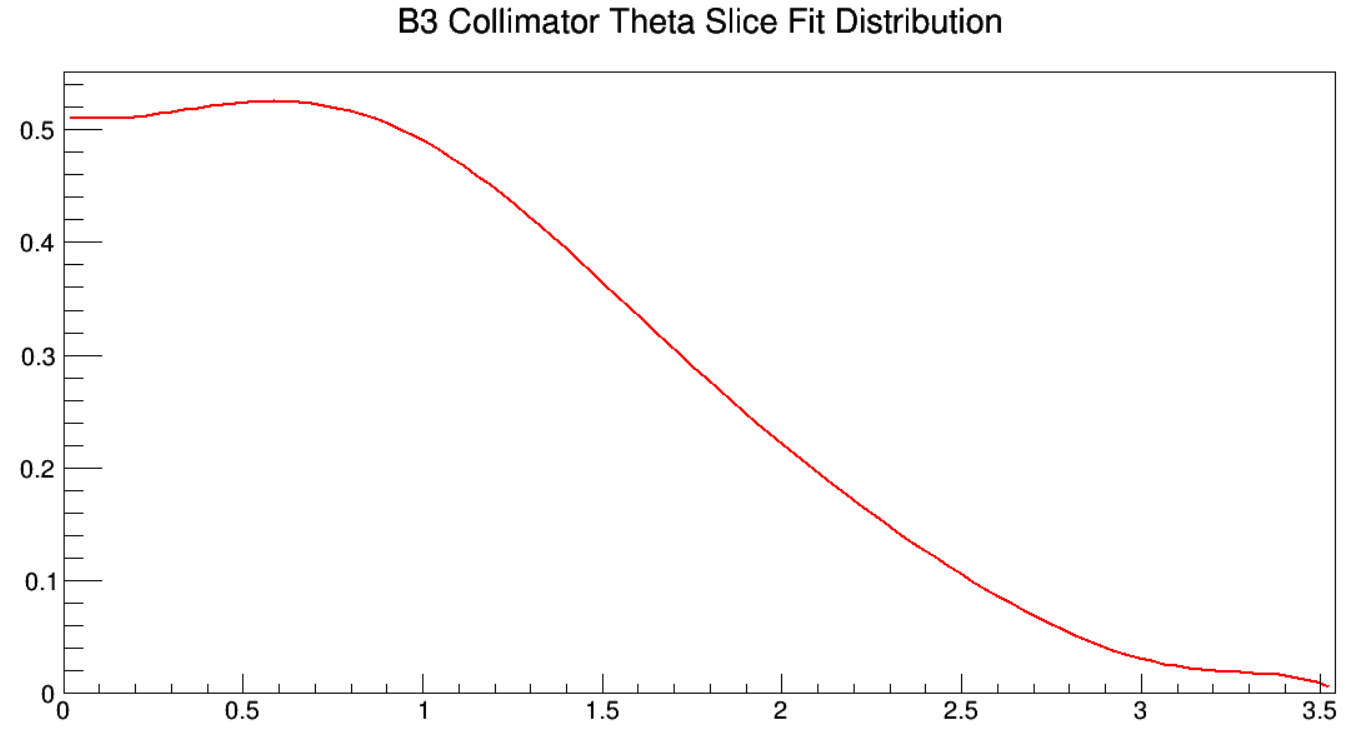
\includegraphics[width=0.49\textwidth]{Figures/B3_collimator_fit.PNG}}\hfill
    \subfloat[]{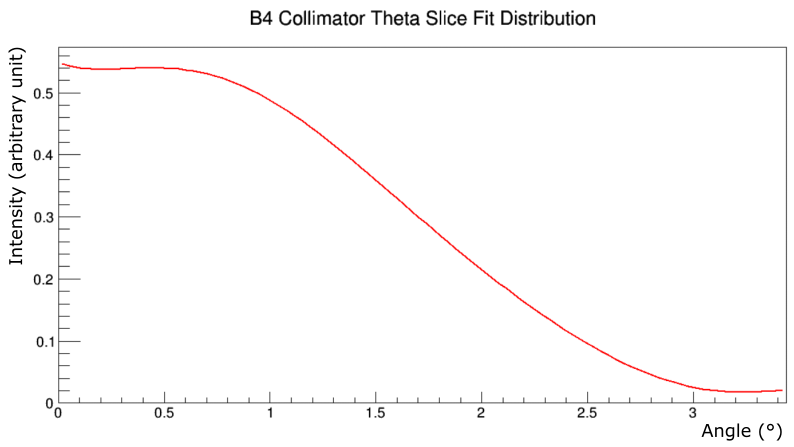
\includegraphics[width=0.49\textwidth]{Figures/B4_collimator_fit.PNG}}\par
    \subfloat[]{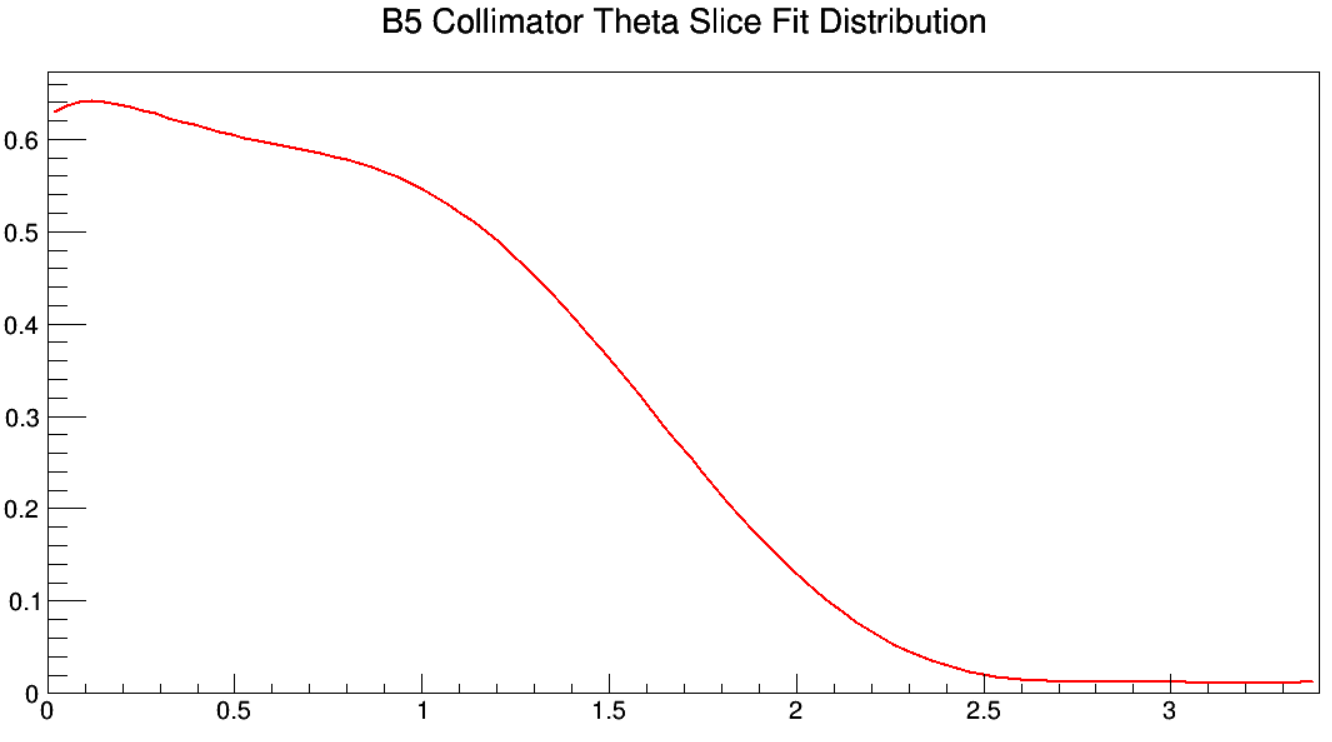
\includegraphics[width=0.49\textwidth]{Figures/B5_collimator_fit.PNG}}

    \caption{Light profiles for the collimator optics provided by the University of Warwick. The profile for each barrel collimator (B1-B5) is shown in (a)-(e) respectively. The light intensity in arbitrary units is shown on the y-axis, while the polar angle of the light is shown on the x-axis.}\label{fig:collimator_TF1}
\end{figure}



\begin{figure}
    \centering
    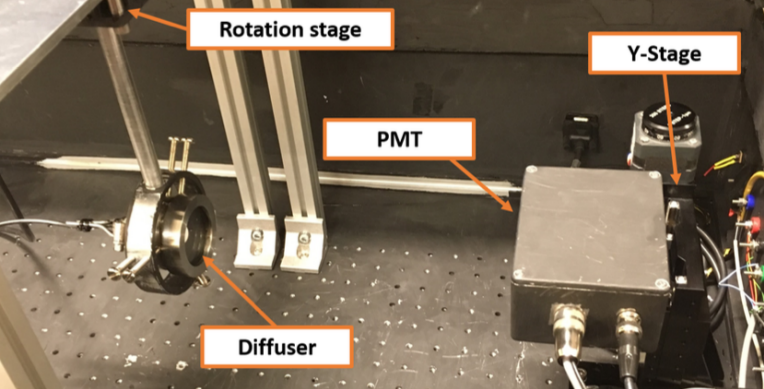
\includegraphics[width=0.7\textwidth]{Figures/diffuser_test_stand.png}
    \caption{Setup of the diffuser test stand provided by the University of Warwick.}
    \label{fig:diffuser_test_stand}
\end{figure}

Figure \ref{fig:diffuser_TF1} shows distributions provided by this test stand data which are preliminary fits made by ROOT to the light profiles for the diffuser. These distributions are not phi-averaged, and instead are scans across the front of the diffuser. The asymmetries in the profile intensities between -40$\degree$ and 0$\degree$ and 0$\degree$ and 40$\degree$ are due to imperfections in the diffuser balls and their enclosures. 

\begin{figure}[!htbp]
    \centering
    
    \caption{Light profiles for the diffuser optics provided by the University of Warwick. The profile for each barrel diffuser (B1-B5) is shown in (a)-(e) respectively. The light intensity in arbitrary units is shown on the y-axis, while the polar angle scan of the light across the diffuser is shown on the x-axis.}\label{fig:diffuser_TF1}
    
    \subfloat[]{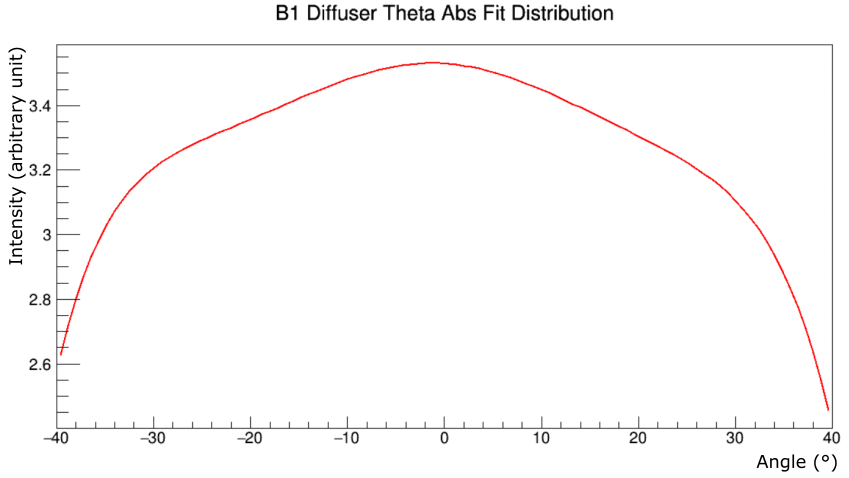
\includegraphics[width=0.49\textwidth]{Figures/B1_diffuser_fit.PNG}}\hfill
    \subfloat[]{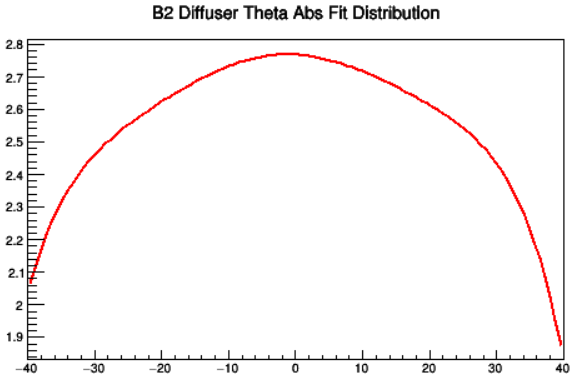
\includegraphics[width=0.49\textwidth]{Figures/B2_diffuser_fit.PNG}}\par
    \subfloat[]{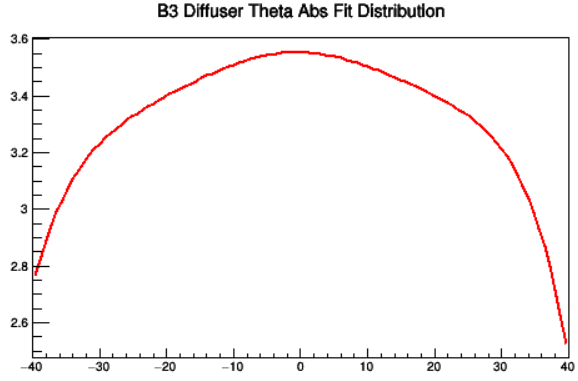
\includegraphics[width=0.49\textwidth]{Figures/B3_diffuser_fit.PNG}}\hfill
    \subfloat[]{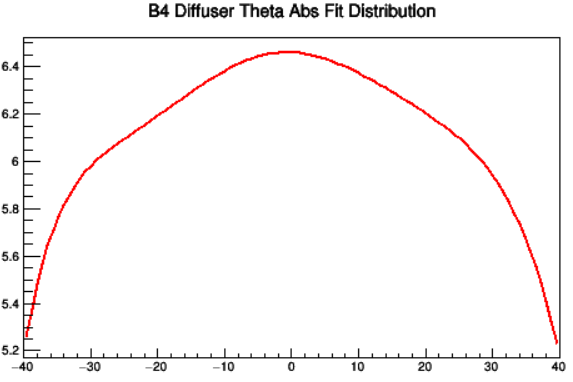
\includegraphics[width=0.49\textwidth]{Figures/B4_diffuser_fit.PNG}}\par
    \subfloat[]{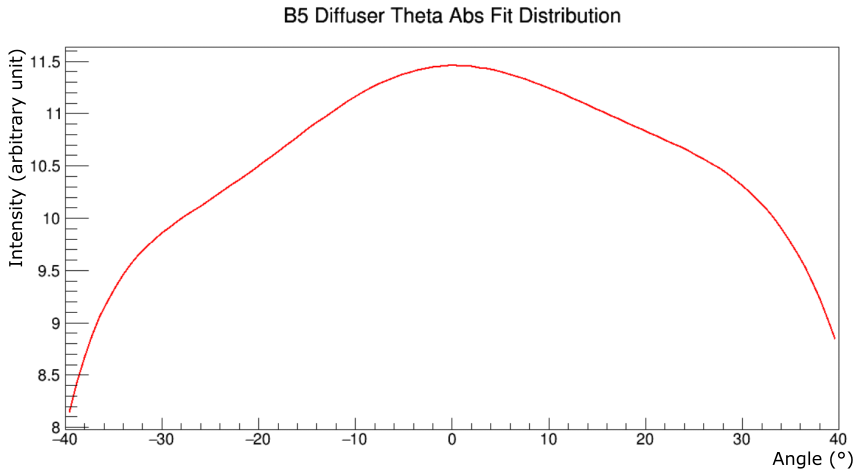
\includegraphics[width=0.49\textwidth]{Figures/B5_diffuser_fit.PNG}}
    
\end{figure}






\section{First commissioning data from UKLI}

In September of 2019 and November of 2019 two sets of test data were taken of the collimator, the diffuser and the bare fibre optic (the B2 bare fibre) and using an event display developed by the University of Warwick, occupancy plots of the test data sets were produced. Figure \ref{fig:occupancy_coll} shows the occupancy plots for the collimator optic from the November 2019 dataset showing the beam spot inside the unrolled volume of the Super-Kamiokande detector. Similarly, Figure \ref{fig:occupancy_diffuser} shows the occupancy plots for the diffuser optic from the November 2019 dataset. The graph in the bottom right hand corner of the occupancy plots show the corrected time-of-flight plots for the PMT hits from the injector. The intensely dark purple hits in Figure \ref{fig:occupancy_diffuser} are ``hot channels'' and have not been accounted for - these should not be mistaken for scattered hits.



\begin{figure}
    \centering
    
    \caption{Occupancy plots for the collimator optics from the UKLI November 2019 test run for each barrel collimator in the unrolled volume of the SK detector. The crosses show the injector positions, and the collimator beam spots are also shown (the PMTs with highest occupancy). The corrected time-of-flight plots for the PMT hits is shown in the bottom right corner.}
    \label{fig:occupancy_coll} 
    \subfloat[B1 collimator]{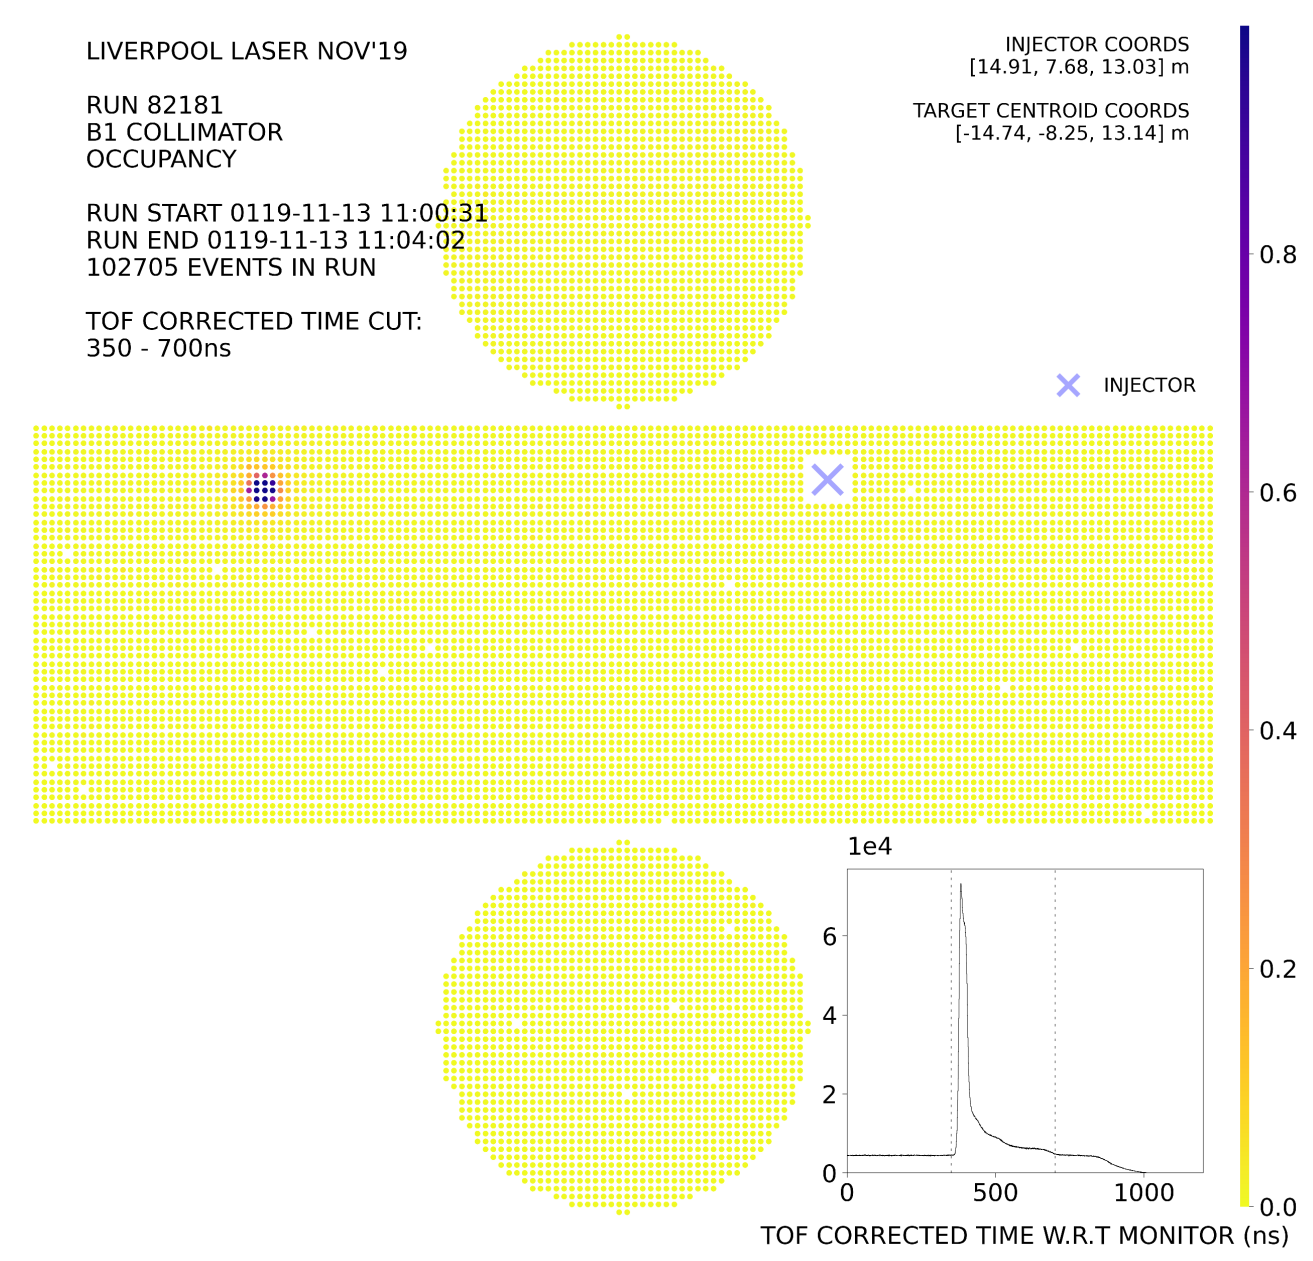
\includegraphics[width=0.49\textwidth]{Figures/B1_occupancy_coll.PNG}} \hfill
    \subfloat[B2 collimator]{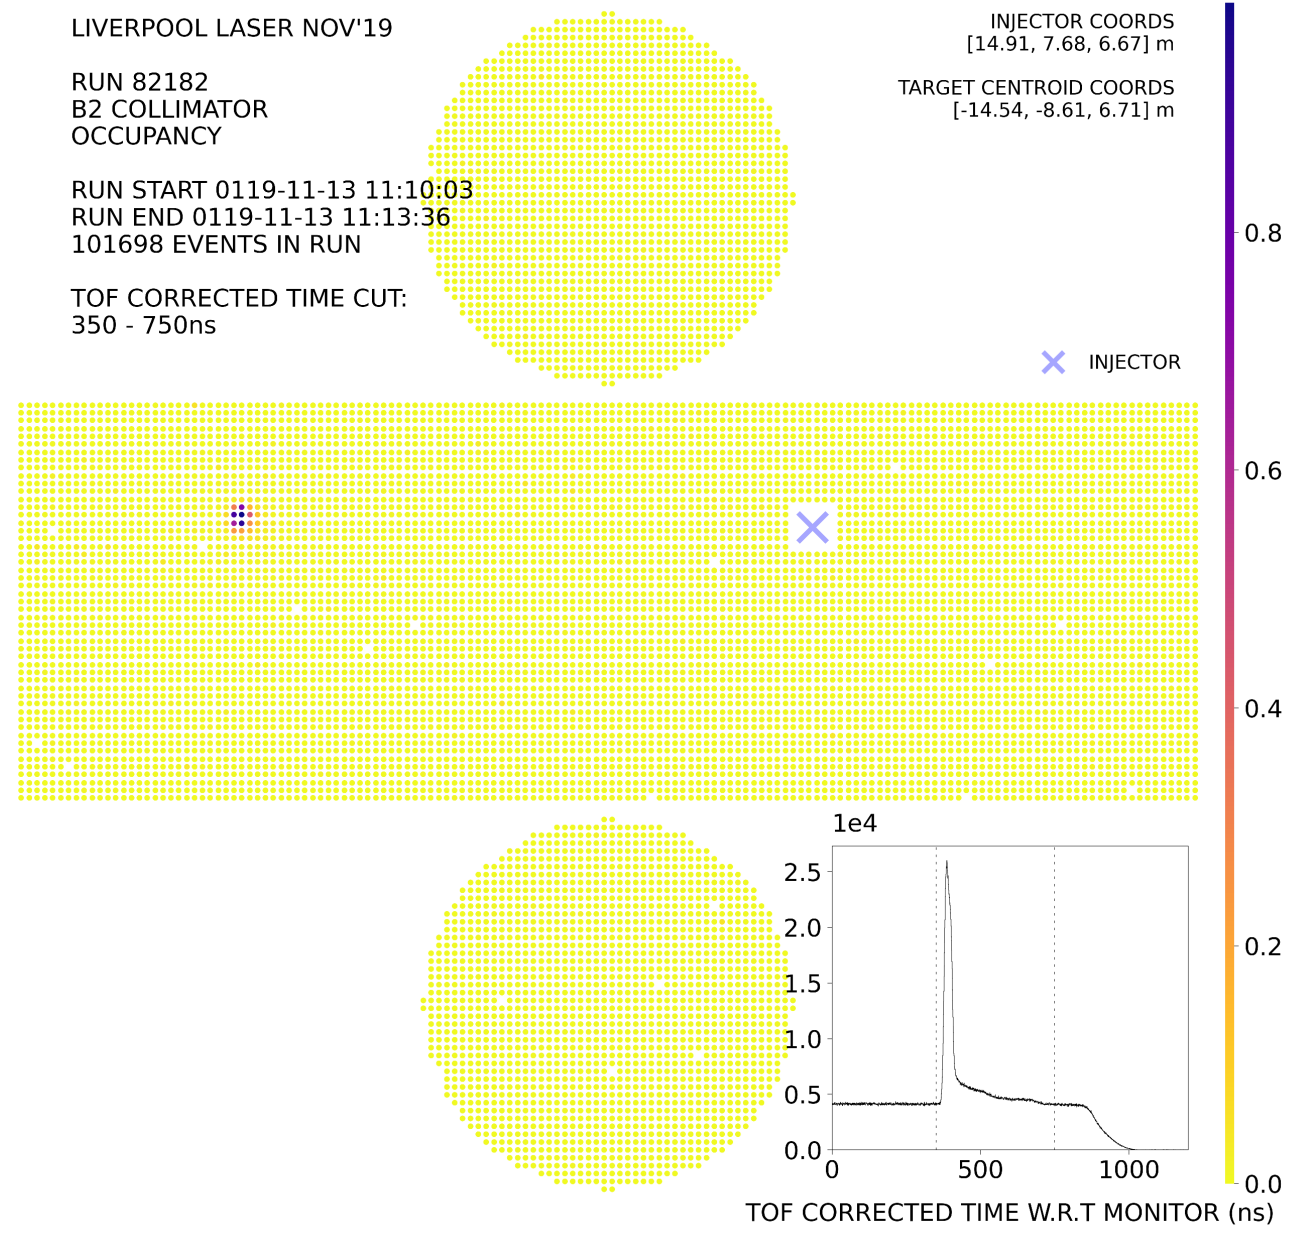
\includegraphics[width=0.49\textwidth]{Figures/B2_occupancy_coll.PNG}} \par
    \subfloat[B3 collimator]{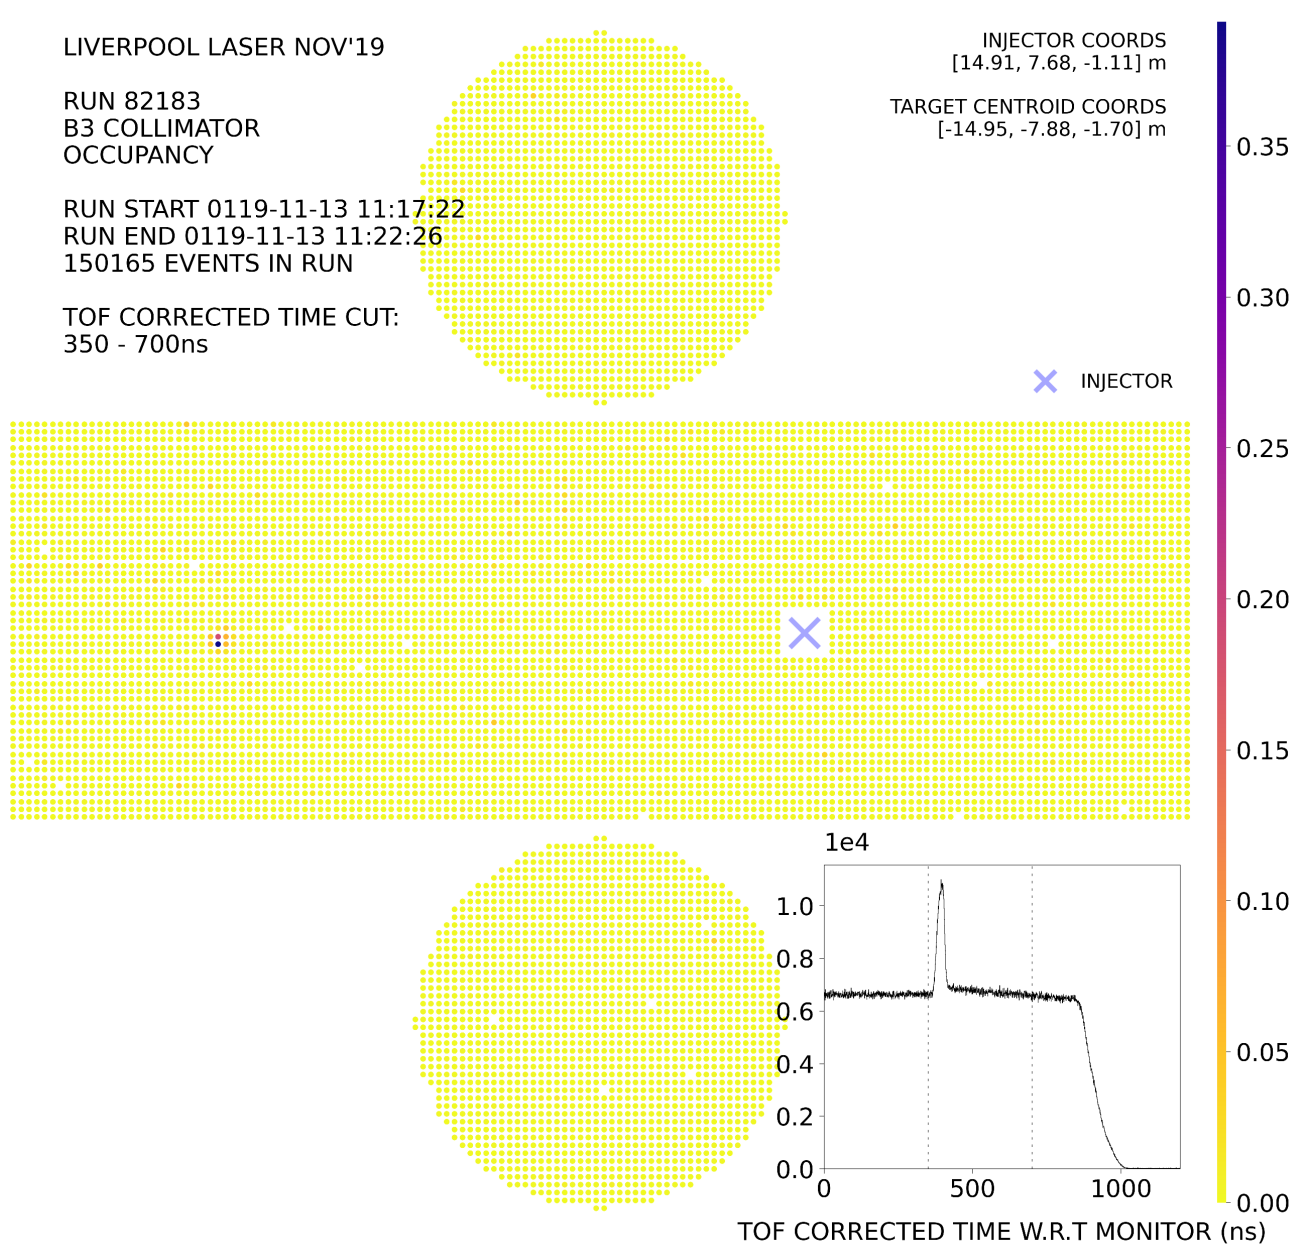
\includegraphics[width=0.49\textwidth]{Figures/B3_occupancy_coll.PNG}} \hfill
    \subfloat[B4 collimator]{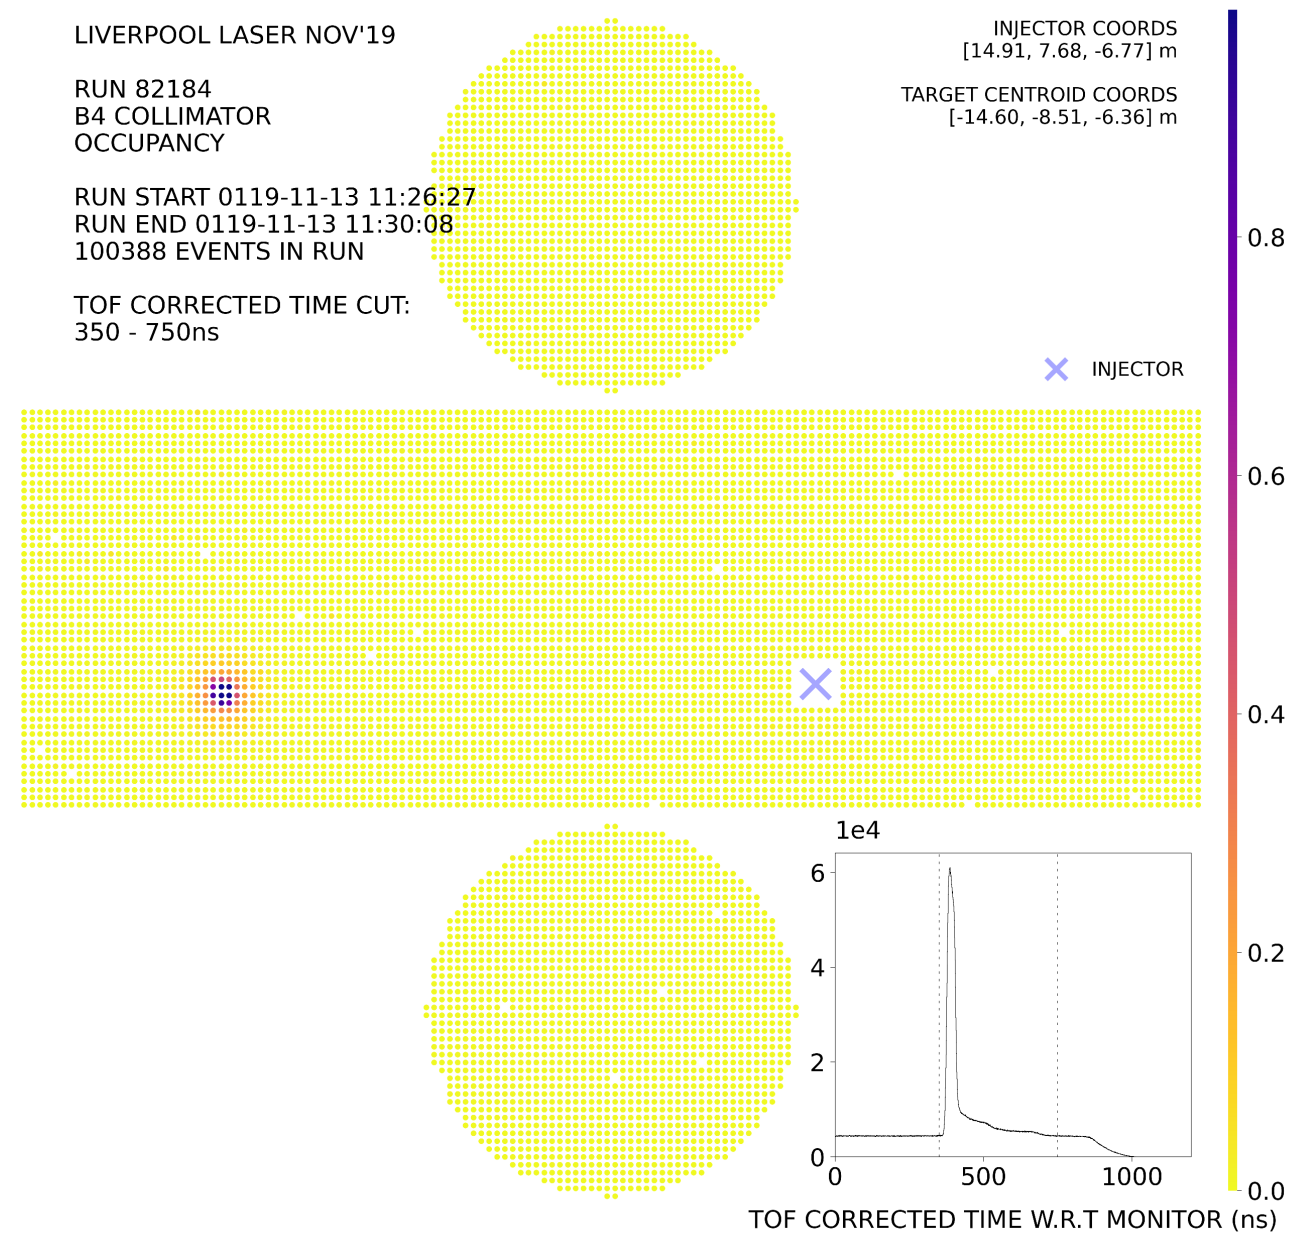
\includegraphics[width=0.49\textwidth]{Figures/B4_occupancy_coll.PNG}} \par
    \subfloat[B5 collimator]{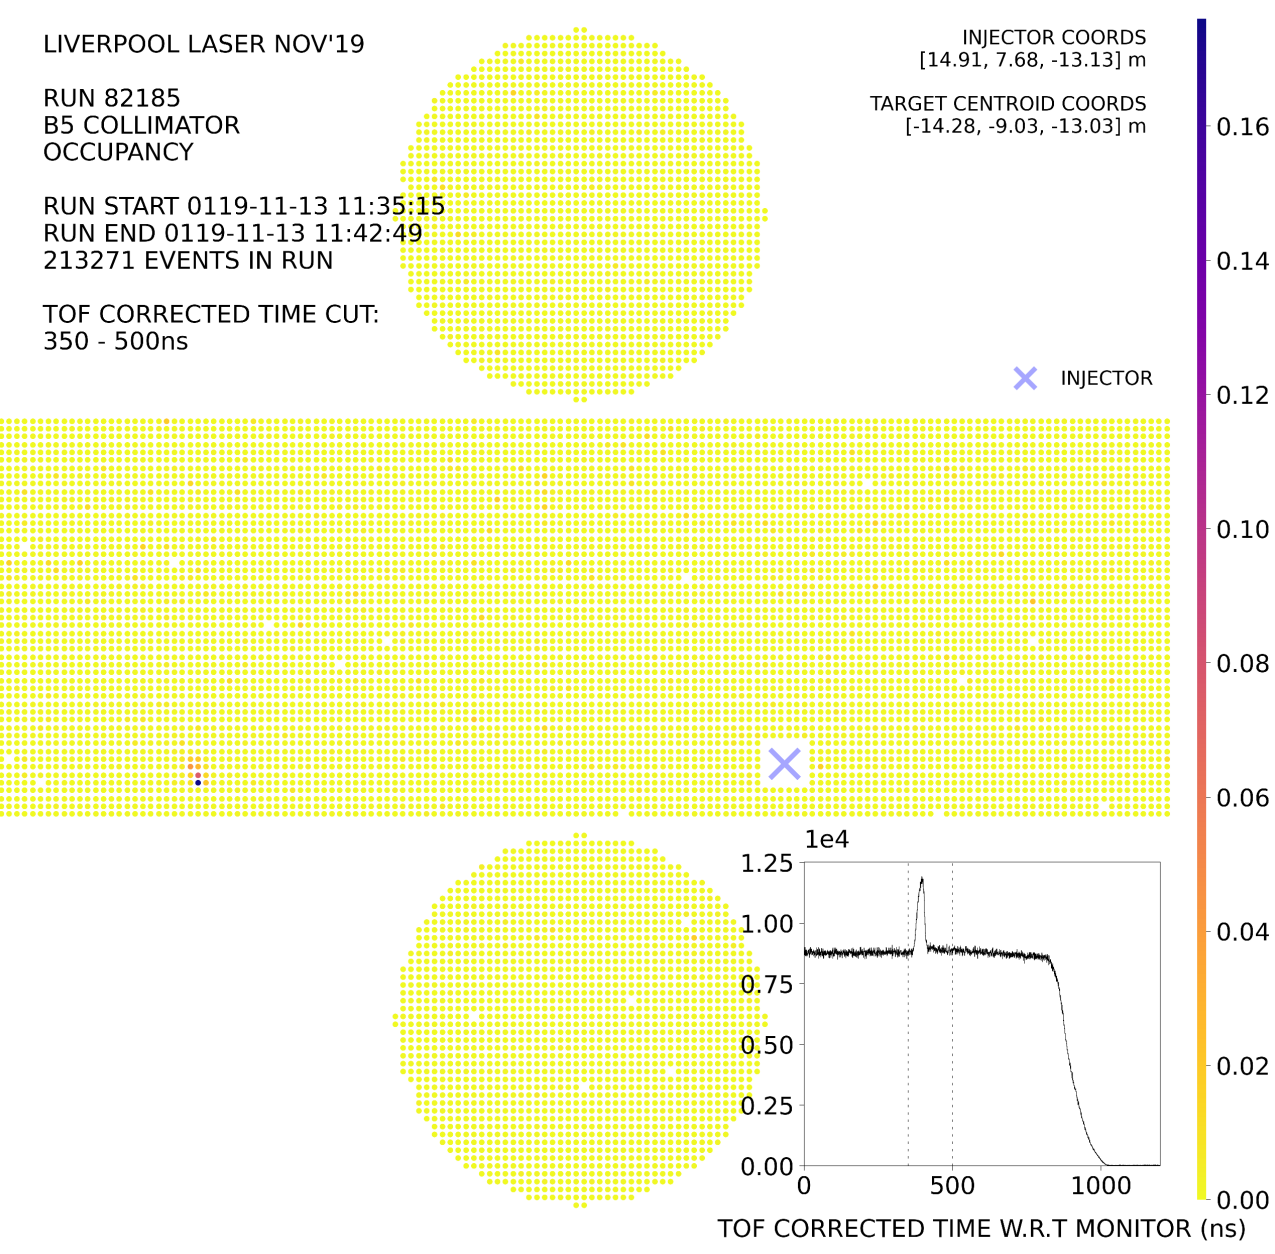
\includegraphics[width=0.49\textwidth]{Figures/B5_occupancy_coll.PNG}}
    \thisfloatpagestyle{empty}
\end{figure}


\begin{figure}
    \centering
    
    \caption{Occupancy plots for the diffuser optics from the UKLI November 2019 test run, where the injector positions are shown by crosses.The corrected time-of-flight plots for the PMT hits is shown in the bottom right corner.} \label{fig:occupancy_diffuser} 
    
    \subfloat[B1 diffuser]{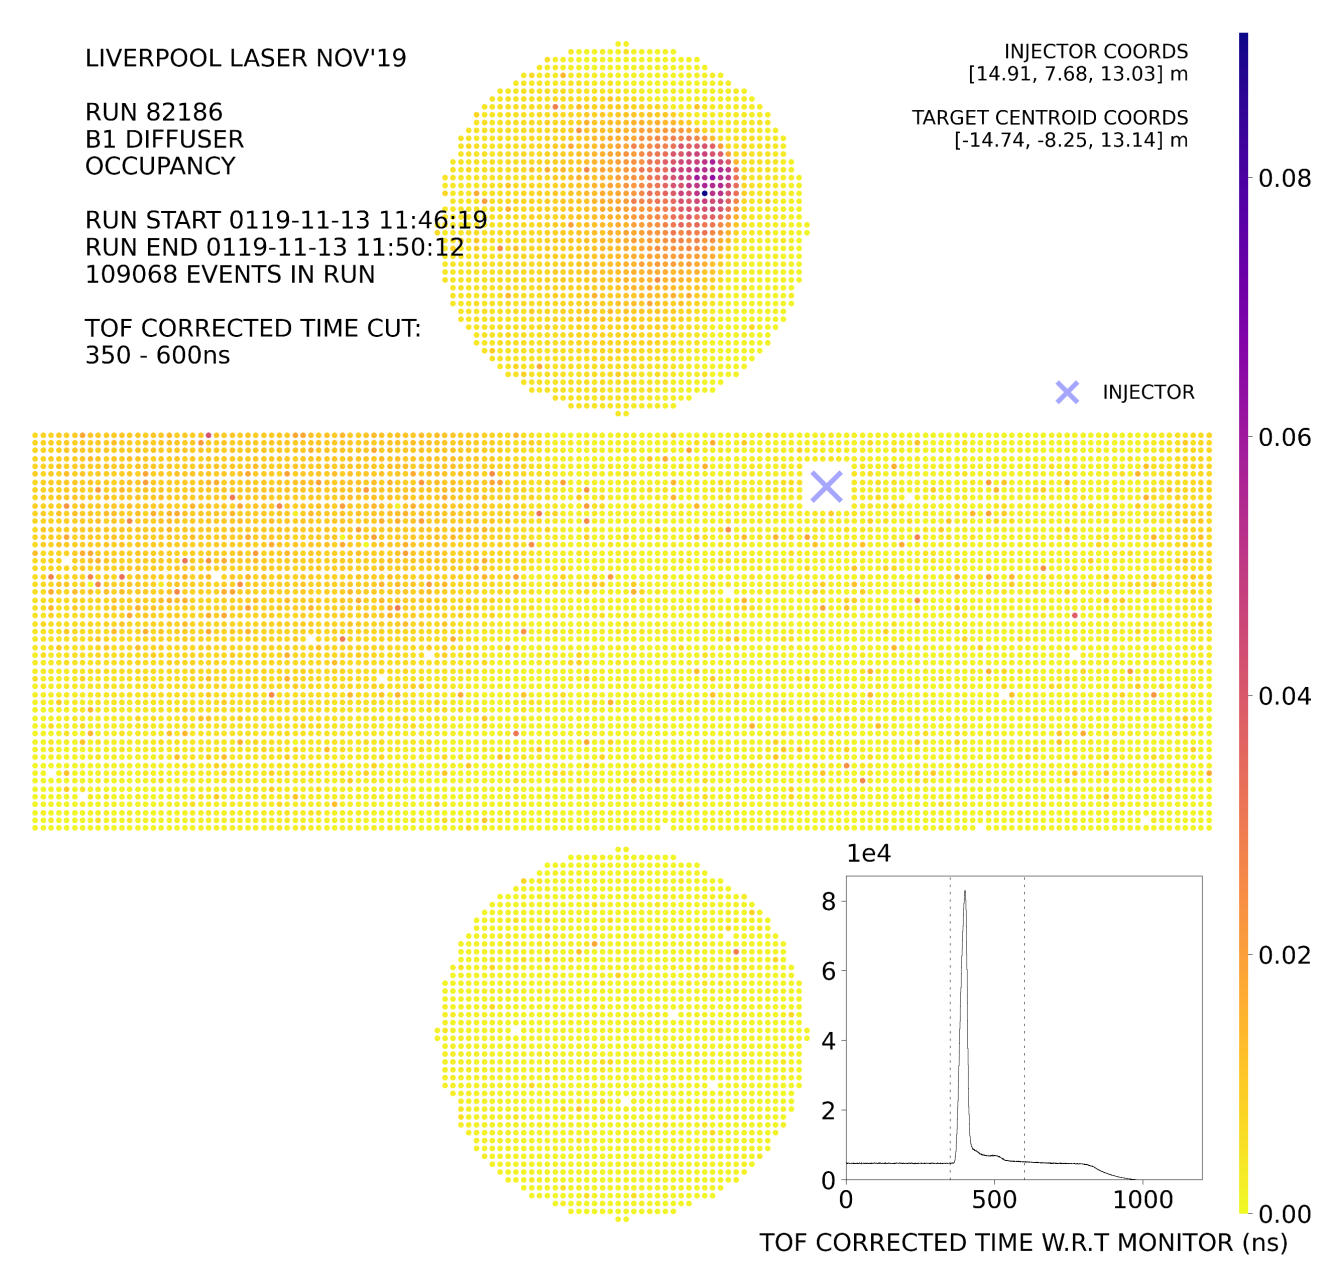
\includegraphics[width=0.49\textwidth]{Figures/B1_occupancy_diff.PNG}} \hfill
    \subfloat[B2 diffuser]{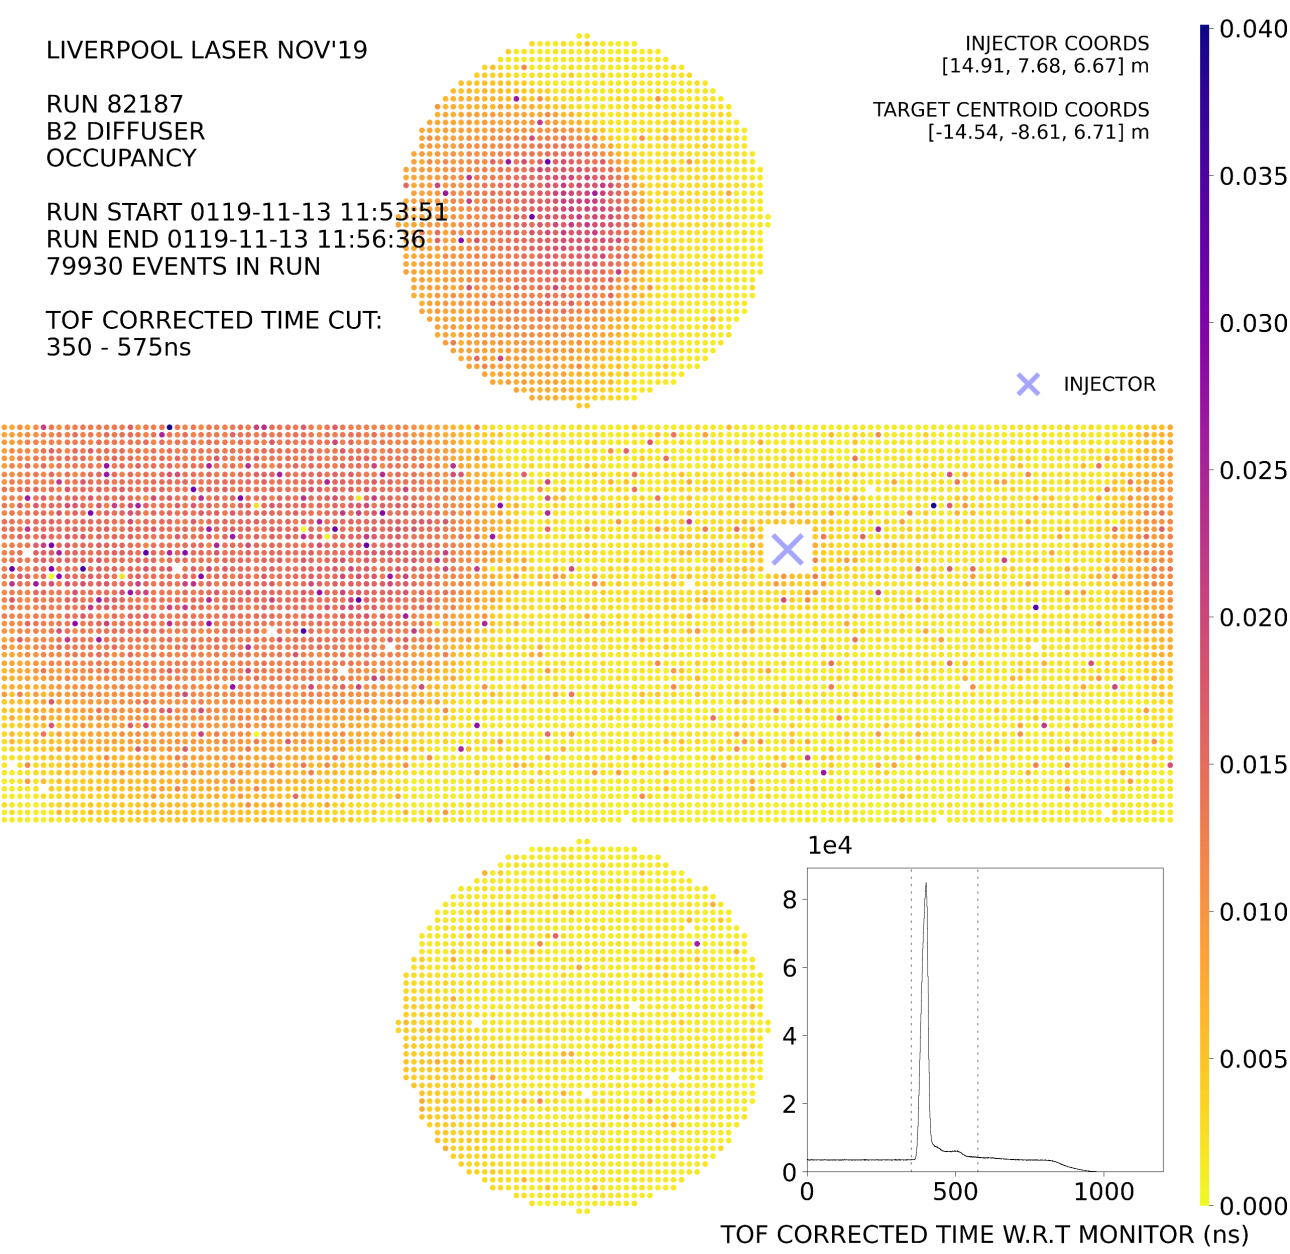
\includegraphics[width=0.49\textwidth]{Figures/B2_occupancy_diff.PNG}} \par
    \subfloat[B3 diffuser]{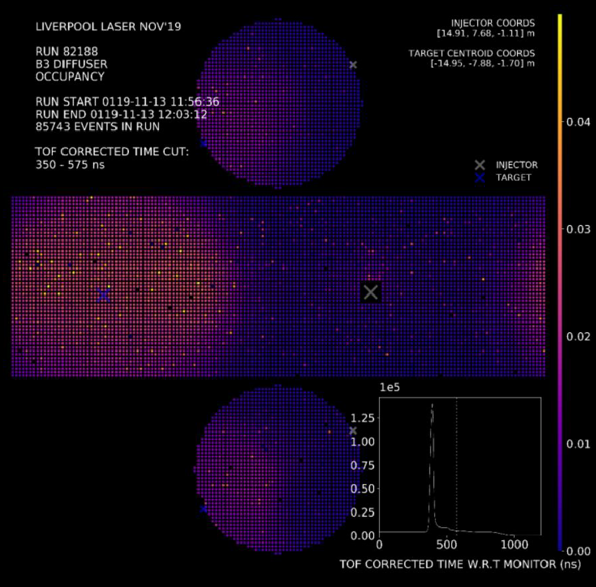
\includegraphics[width=0.49\textwidth]{Figures/B3_occupancy_diff.PNG}} \hfill
    \subfloat[B4 diffuser]{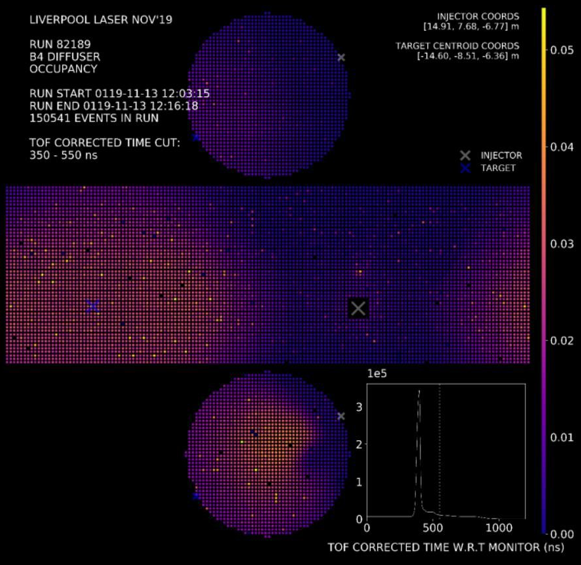
\includegraphics[width=0.49\textwidth]{Figures/B4_occupancy_diff.PNG}} \par
    \subfloat[B5 diffuser]{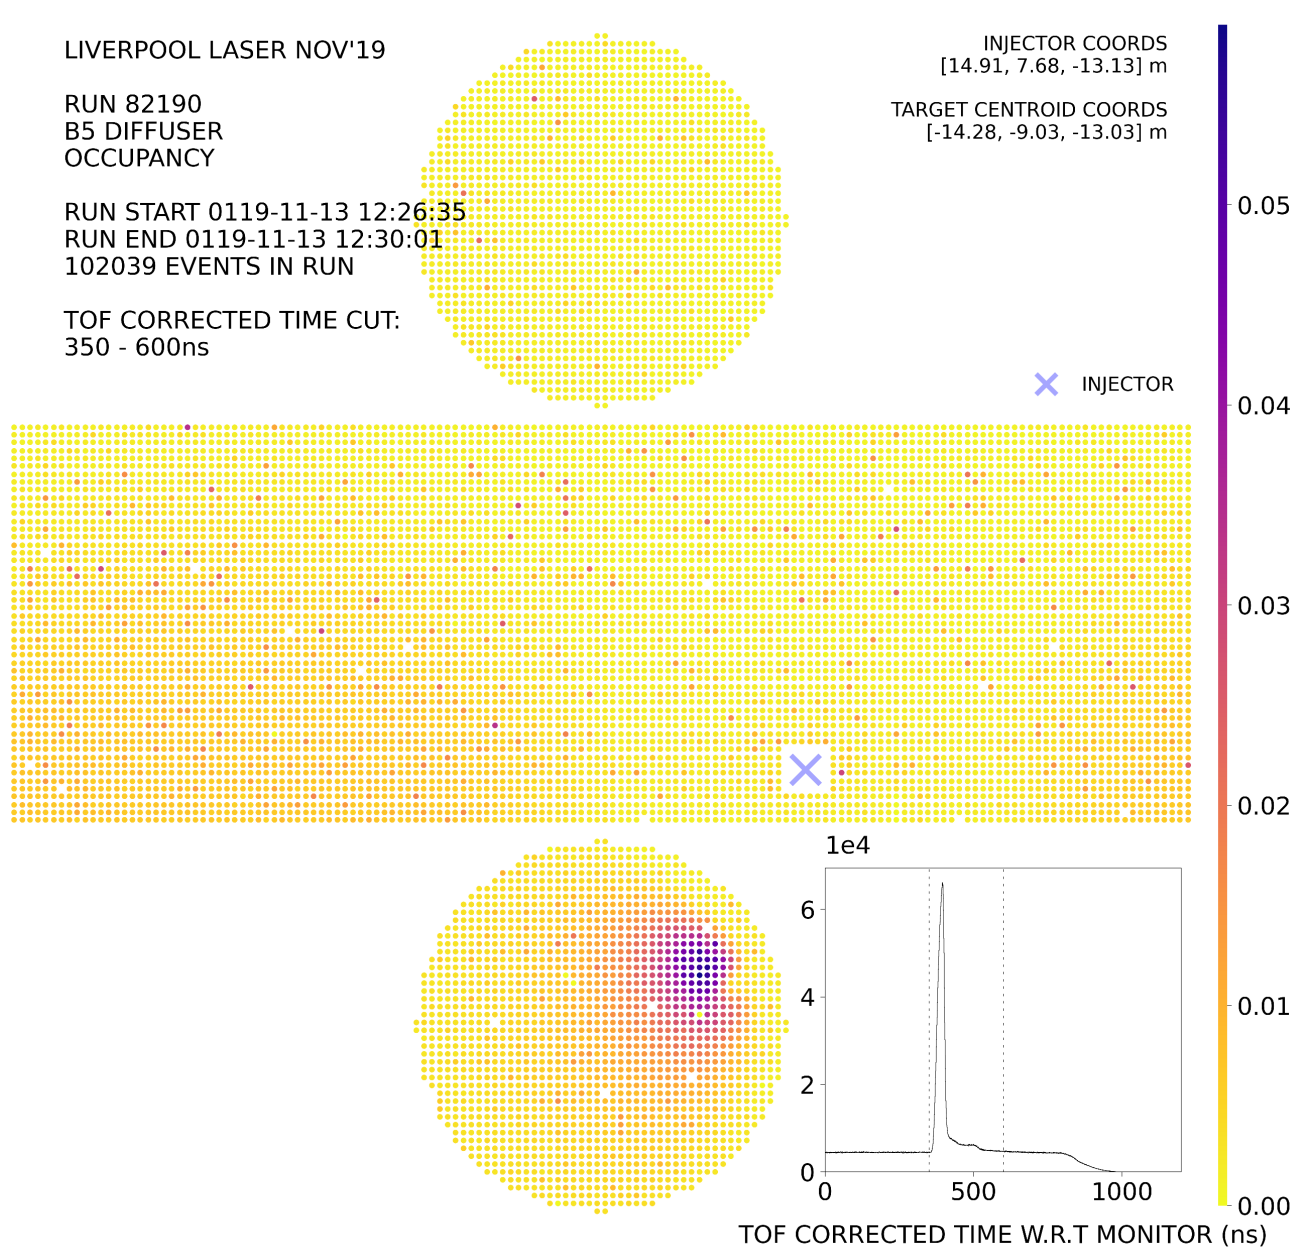
\includegraphics[width=0.49\textwidth]{Figures/B5_occupancy_diff.PNG}}
    
\end{figure}

The UKLI was also added to the ``autocalib'' system used for long term monitoring of the water parameters in Super-Kamiokande by the Korean laser system. In early 2020 the autocalib scheduler was modified to incorporate data taking by the UKLI system which was very useful for gadolinium loading calibration purposes but also in the longer term, it will be useful in the monitoring of daily/weekly water coefficient property measurements, investigation of depth dependence with respect to the water properties and PMT property calibration. Figure \ref{fig:autocalib} shows the schedule for autocalib, and the black dashed lines show the position of the UK barrel collimator and diffusers with respect to the other autocalib data taking streams. The horizontal blue line shows the length of the one autocalib cycle, which is about 4.6 seconds, with each UKLI optic taking about 3310 events per day. 

\begin{figure}
    \centering
    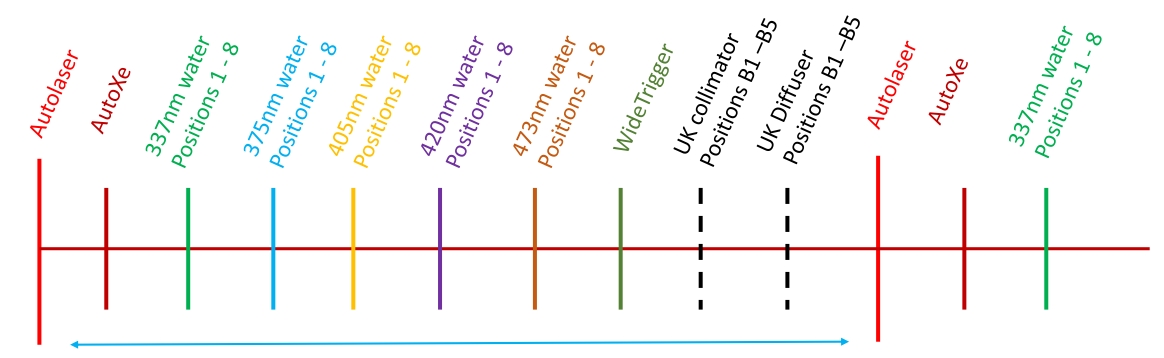
\includegraphics[width=0.8\textwidth]{Figures/autocalib.png}
    \caption{Schematic showing position of the UKLI in autocalib scheduler: the black dashed lines show the UKLI B1-B5 collimator and diffuser optics and the horizontal blue line shows the length of one autocalib cycle.}
    \label{fig:autocalib}
\end{figure}

Figures \ref{fig:B1_coll_auto_July} and \ref{fig:B1_diff_auto_July} show the occupancy plots for autocalib data taken in July 2020, for the B1 collimator and the B1 diffuser respectively. From this point onwards all plots relating to the B2 - B5 injectors for both the collimators and diffusers will be shown in Appendix A. As can be seen in the text in the upper left hand corner, the number of events in the run is a lot less than the 100,000 events or so taken in the test runs, however they are more than sufficient for monitoring purposes.


\begin{figure}
    \centering
    
    \begin{minipage}{0.47\textwidth}
        \centering
        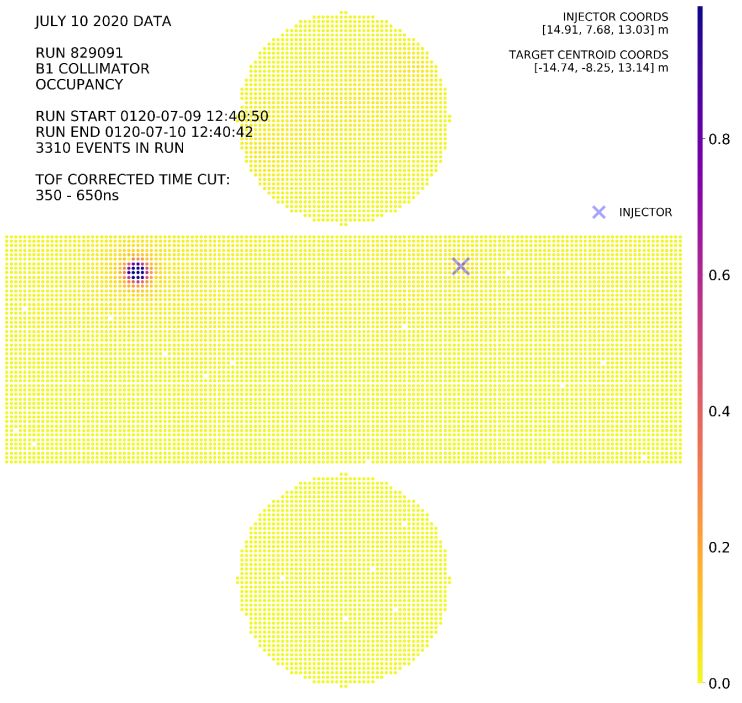
\includegraphics[width=\textwidth]{Figures/B1_occupancy_coll_auto.PNG} % first figure itself
        \caption{Occupancy plot for the B1 collimator optic from the UKLI Autocalib July 2020 run.}
        \label{fig:B1_coll_auto_July}
    \end{minipage}\hfill
    \begin{minipage}{0.47\textwidth}
        \centering
        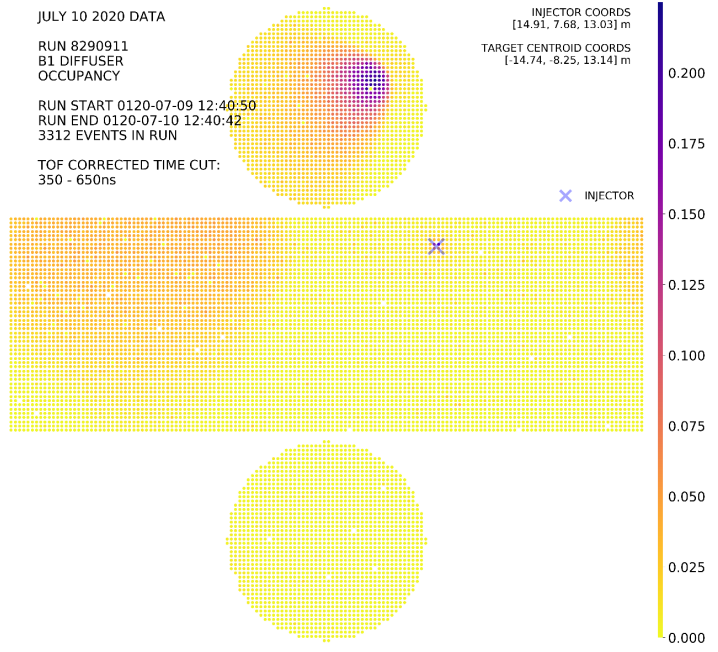
\includegraphics[width=\textwidth]{Figures/B1_occupancy_diff_auto.PNG} % second figure itself
        \caption{Occupancy plot for the B1 diffuser optic from the UKLI Autocalib July 2020 run.}
        \label{fig:B1_diff_auto_July}
    \end{minipage}
\end{figure}


\section{Implementation of UKLI in SK Simulation}
In order to simulate the data taken with the UKLI, SKDETSIM \cite{harada2019development}, the Super Kamiokande Detector Simulator was used. SKDETSIM uses GEANT3 (GEometry ANd Tracking 3 \cite{geant3_cite}) to simulate what the particles in each event would do inside the detector, and tracks the particle's trajectories and energy loss. Simulating the light injection from the UKLI system in SKDETSIM was done in a similar way to the Korean method of producing Monte Carlo: the same versions of the calibration scripts were used, however, small modifications were made to them and to the version of SKDETSIM used to simulate the input photons from the system in the detector. The calibration software allows for the number of events and the number of injected photons to be set, in order to generate many Monte Carlo files with varying absorption, Rayleigh and Mie scattering parameters. 
\newline
Along with making sure the position of the injectors was set to that of the UKLI injectors (shown in Table \ref{table:UKLI_loc}), the opening angle of the injectors determined by the simulation had to be set to accomodate the fact that the injectors for the UKLI system now consisted of three different opening angles for the collimator, diffuser and bare fibre optics. Previously, to set the angle of the photons in the beam, a parameter relating to the width of the input injector beam was produced using a Gaussian random number generator to output the photon angle. However, an entirely new method of determining the opening angle of the beam was needed to include the information from the light profiles taken from the test stands at Warwick. 

\begin{table}
\centering
\begin{tabular}{||c|c|c|c|c||}
    \hline UKLI Barrel Injector & $\mathrm{x}(\mathrm{cm})$ & $\mathrm{y}(\mathrm{cm})$ & $\mathrm{z}(\mathrm{cm})$ & Misalignment angle $\left({ }^{\circ}\right)$ \\
    \hline B1 & 1490.73 & 768.14 & 1224.0 & 4.1 \\
    \hline B2 & 1490.73 & 768.14 & 742.0 & 3.5 \\
    \hline B3 & 1490.73 & 768.14 & -200.0 & 3.4 \\
    \hline B4 & 1490.73 & 768.14 & -747.0 & 6.3 \\
    \hline B5 & 1490.73 & 768.14 & -1413.0 & - \\
    \hline 
\end{tabular}
\caption{Beam spot positions (x,y,z) of the UKLI injectors in cm and misalignment of the injectors in degrees.} 
\label{table:UKLI_loc}
\end{table}

In order to validate the positions of the targets for the UKLI system, and the relationship between the width of the beam and the output angle, producing charge weighted histograms from UKLI test runs is very helpful. It allows us to explore the shape of the beam profile and intensity. Figures \ref{fig:charge_weighted_nov_sept_B1} and \ref{fig:charge_weighted_nov_sept_B4} shows the charge weighted z-profiles for the September and November 2019 datasets for the B1 and B4 collimator injectors, where the blue dashed line shows the expected target position. These are produced by selecting hit PMTs which are greater than 2 m away from the injector (to avoid including PMT hits from backscattered light), and filling the histogram with the z-position of the hit PMT and the number of hits the hit PMT receives multiplied by the corrected charge from the PMT. The corrected PMT charge ($q_{corrected}$) is calculated using Equation \ref{eq:gain_correction}, where $q$ is the charge, and the gain correction value ($gain$) is taken from official Super-Kamiokande gain tables. By fitting these charge weighted histograms with a gaussian and calculating its mean value (i.e. the actual target location), it was possible to calculate the deviation from the expected target location given in the simulation (the dashed blue lines in Figures \ref{fig:charge_weighted_nov_sept_B1} and \ref{fig:charge_weighted_nov_sept_B4}), and then using simple trigonometry the misalignment angle of the injector was calculated, as shown in Table \ref{table:UKLI_loc}.

\begin{equation}
   q_{corrected} = q/(1 + gain)
\label{eq:gain_correction}
\end{equation}

\begin{figure}
    \centering
    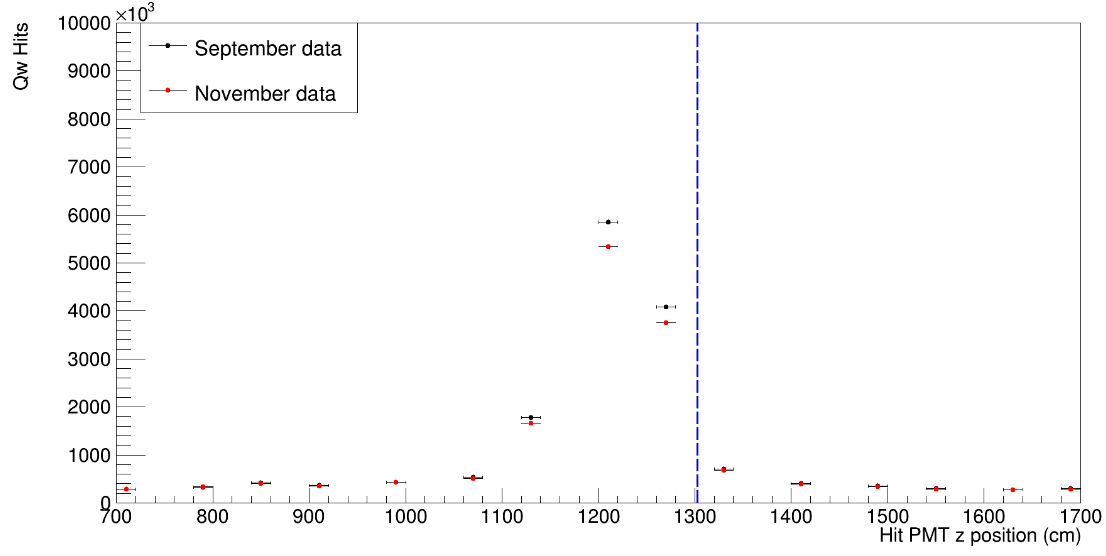
\includegraphics[width=0.9\textwidth]{Figures/charge_weighted_nov_sept_B1.PNG}
    \caption{Charge weighted z profile plots for the B1 collimator UKLI injector optic, with the September 2019 test run data shown in black and the November 2019 test run data shown in red.}
    \label{fig:charge_weighted_nov_sept_B1}
\end{figure}

\begin{figure}
    \centering
    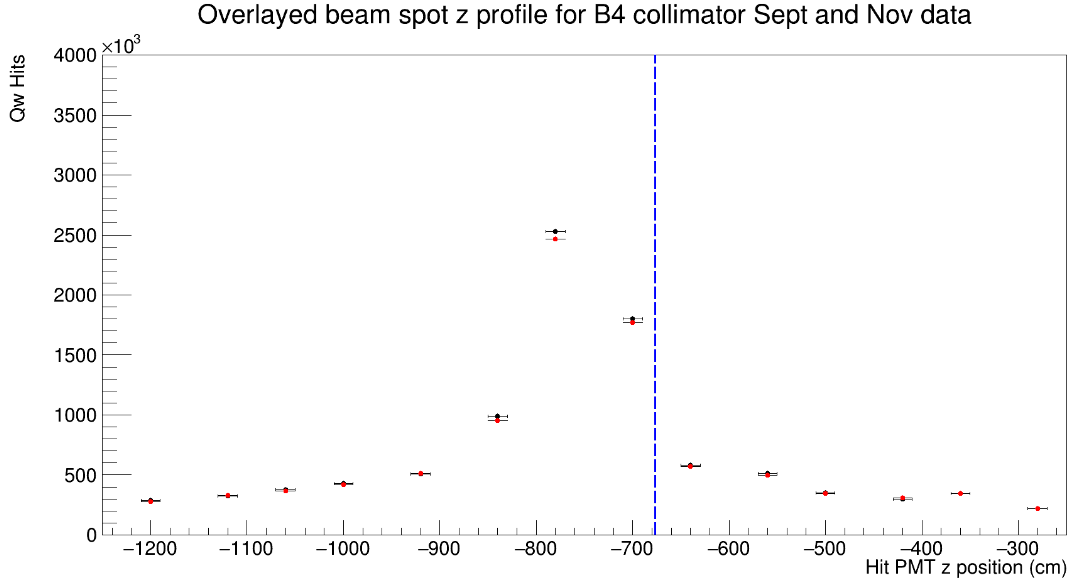
\includegraphics[width=0.9\textwidth]{Figures/charge_weighted_nov_sept_B4.PNG}
    \caption{Charge weighted z profile plots for the B4 collimator UKLI injector optic, with the September 2019 test run data shown in black and the November 2019 test run data shown in red.}
    \label{fig:charge_weighted_nov_sept_B4}
\end{figure}


The profiles from the Warwick optic test stands (shown in Figures \ref{fig:collimator_TF1} and \ref{fig:diffuser_TF1}) are then used in the production of the opening angle of the injectors in the detector simulation. This was done by treating the profiles in Figures \ref{fig:collimator_TF1} and \ref{fig:diffuser_TF1} as Probablity Distribution Functions (PDFs) and using inverse transform sampling to make the detector simulation sample at random from it. Inverse transform sampling is a method for generating random numbers from any probability distribution by using the inverse of its cumulative distribution $F^{-1}(x)$. For continuous distributions, such as the results from the collimator and diffuser optics test stands, the algorithm for inverse transform sampling is simple. Firstly, a random variable $U$ is uniformly distributed between [0,1], and secondly the relation $X = F^{-1}_{x}(U)$ would then produce a distribution $X$ following the original probability distribution function, i.e. that of the original PDFs from the optics test stands. 

The first step is to produce the CDFs (cumulative distribution functions) from the PDFs from the optic test stand profile tests. Figure \ref{fig:collimator_TF1} shows that the original fits to the collimator data did not reach 4 degrees, and as a result the PDFs produced needed to be linearly extrapolated from 3.5 degrees where the measurements cut off to reach 4 degrees. Figure \ref{fig:PDF_CDF_coll_B1} shows the PDFs and CDFs produced from the B1 collimator data and Figure \ref{fig:PDF_CDF_diff_B1} shows them for the B1 diffuser data. The CDFs are normalised with a max of one using min-max scaling.


\begin{figure}
    \centering
    
    \begin{subfigure}{0.5\textwidth}
        \centering
        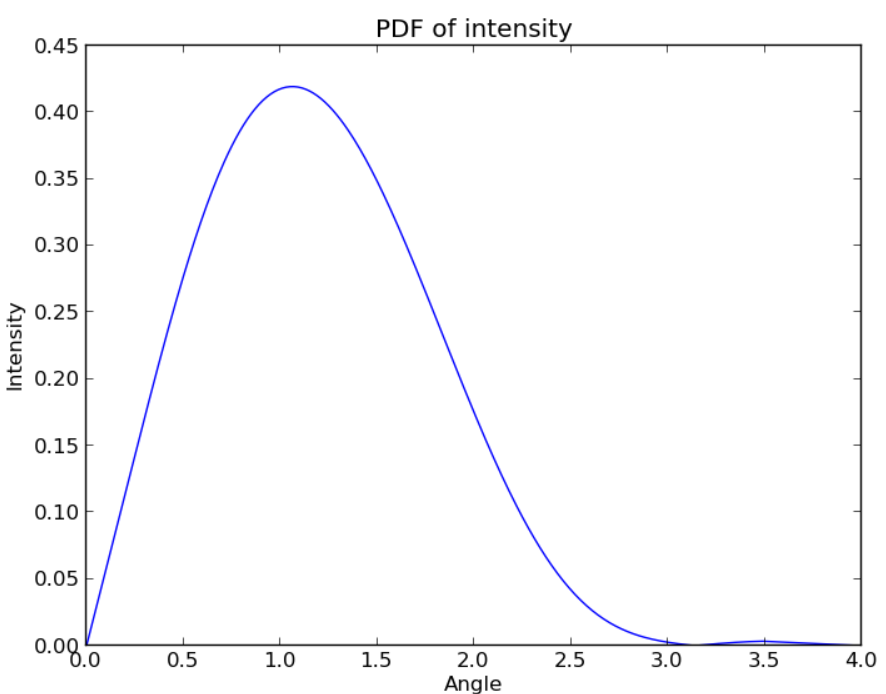
\includegraphics[width=\textwidth]{Figures/B1_coll_pdf.png} % first figure itself
        \caption{PDF for the B1 collimator}
    \end{subfigure}\hfill
    \begin{subfigure}{0.5\textwidth}
        \centering
        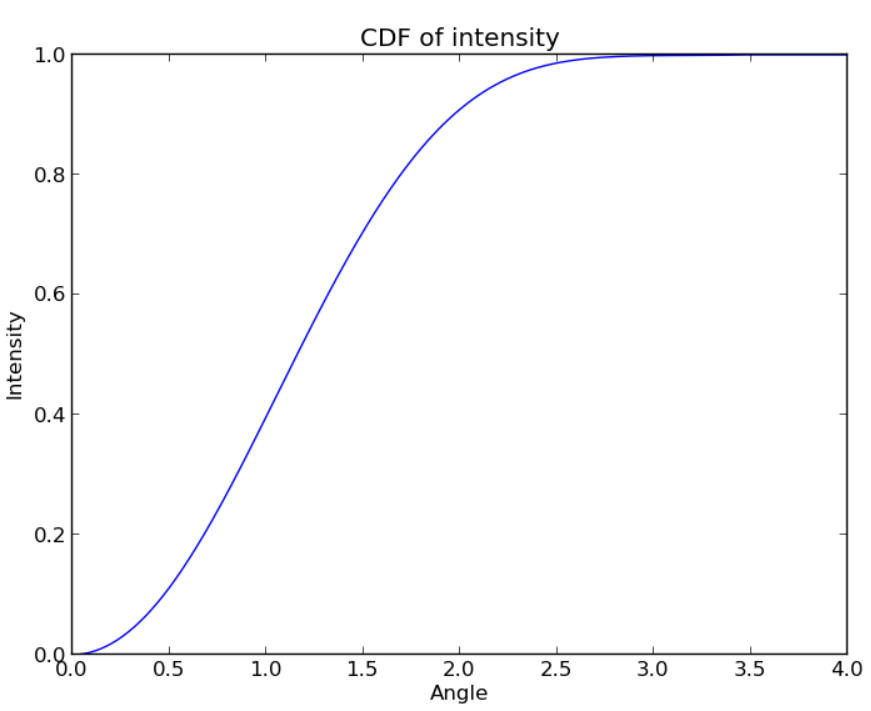
\includegraphics[width=\textwidth]{Figures/B1_coll_cdf.png} % second figure itself
        \caption{CDF for the B1 collimator}
    \end{subfigure}
    \caption{PDF (left) and CDF (right) for the B1 collimator }
    \label{fig:PDF_CDF_coll_B1}
\end{figure}

\begin{figure}
    \centering
    
    \begin{subfigure}{0.5\textwidth}
        \centering
        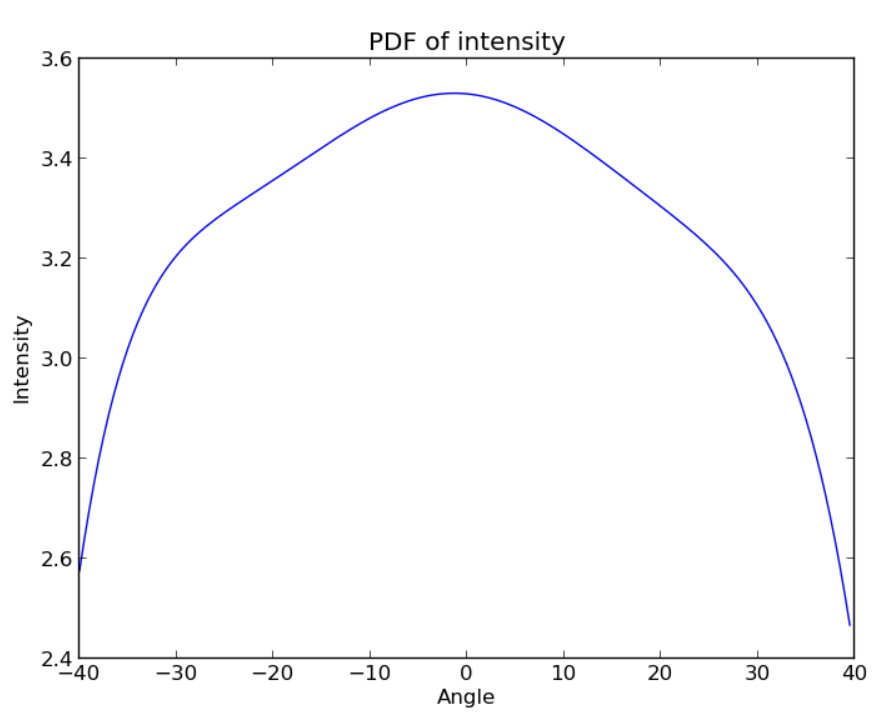
\includegraphics[width=\textwidth]{Figures/B1_diff_pdf.png} % first figure itself
        \caption{PDF for the B1 diffuser}
    \end{subfigure}\hfill
    \begin{subfigure}{0.5\textwidth}
        \centering
        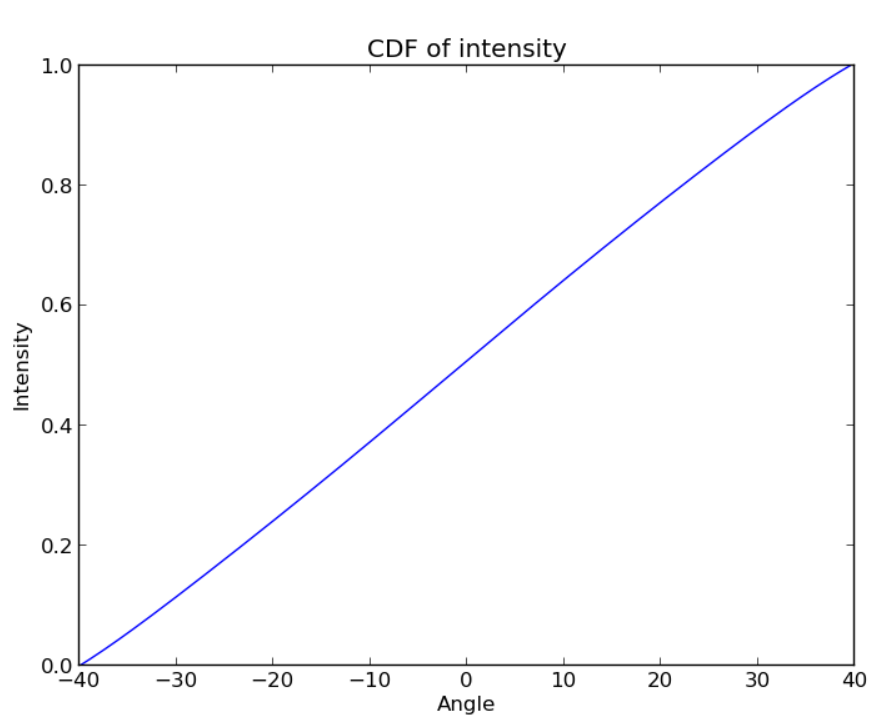
\includegraphics[width=\textwidth]{Figures/B1_diff_cdf.PNG} % second figure itself
        \caption{CDF for the B1 diffuser}
    \end{subfigure}
    \caption{PDF (left) and CDF (right) for the B1 diffuser}
    \label{fig:PDF_CDF_diff_B1}
\end{figure}


After producing the normalised CDFs, the inverse of these CDFs are calculated - Figure \ref{fig:B1_PDF_CDF_inv_diff_coll} shows the comparison of the normalised CDF data for the B1 collimator and diffuser (top sublots, shown in blue) and the polynomial fit to the CDF for the B1 collimator (top subplots, shown in red), and the inverse CDF function (bottom subplots shown in green) and the polynomial fit to this inverse CDF function (bottom subplots shown in purple). 

\begin{figure}
    \centering
    \begin{subfigure}{0.5\textwidth}
        \centering
        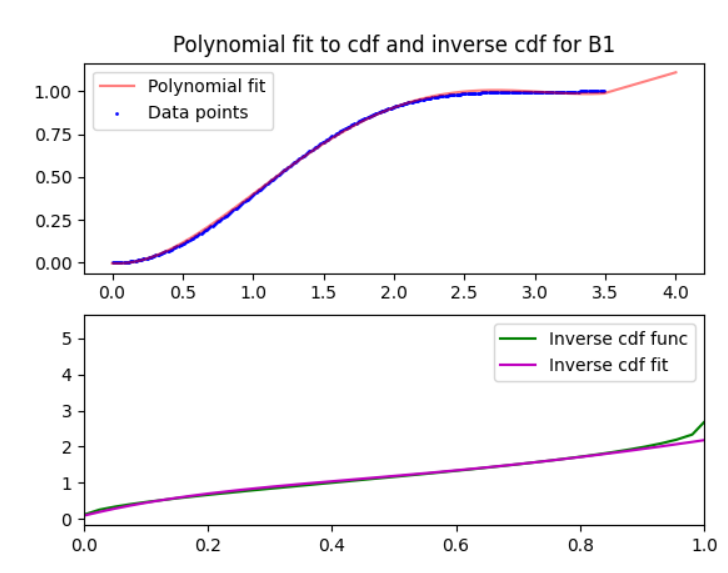
\includegraphics[width=\textwidth]{Figures/B1_inv_coll_cdf.png} % first figure itself
    \end{subfigure}\hfill
    \begin{subfigure}{0.5\textwidth}
        \centering
        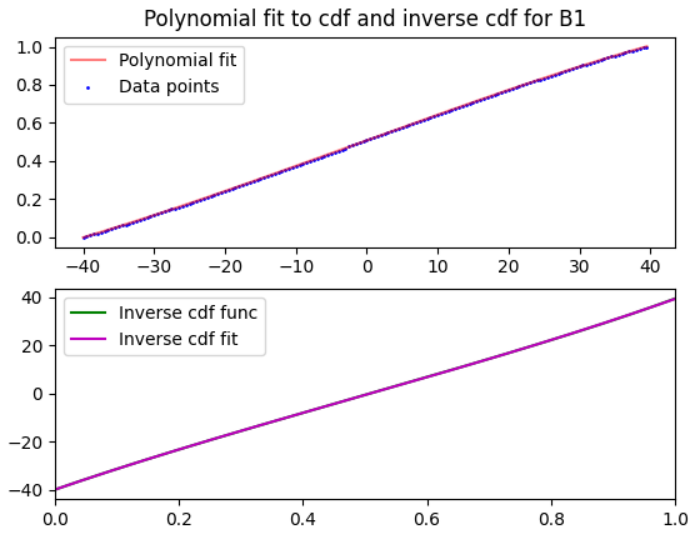
\includegraphics[width=\textwidth]{Figures/B1_inv_diff_cdf.png} % second figure itself
    \end{subfigure}
    \caption{CDF and inverse CDF for the B1 collimator (left) and for the B1 diffuser (right). The y-axis (range 0.0-1.0) on the top subplots for both figures shows the CDF values for the data (blue) and polynomial fit (red) while the x-axis for the top subplots shows the angle scan range for the specific optic in degrees. For the bottom subplots which show the resulting inverse CDF function (green) and fit to this function (purple) these axes are reversed.}
    \label{fig:B1_PDF_CDF_inv_diff_coll}
\end{figure}


After producing the fits to the inverse cumulative distribution functions, these functions were inputted into the detector simulation, SKDETSIM. Using the same event display used to produce the occupancy plots for the autocalib data and the test run data, occupancy plots of the Monte Carlo were produced. These are shown for the B1 collimator and B1 diffuser in Figure \ref{fig:ukli_mc_diff_coll}. These MC were produced with the standard optical settings used for SKDETSIM. Because the original profiles from the test stands were taken in air, adjustments were made so that the refractive index of the water in the detector is taken into account when implementing the inverse CDFs into the detector simulation. 

\begin{figure}[htp]
    \begin{subfigure}{0.49\columnwidth}
    \centering
    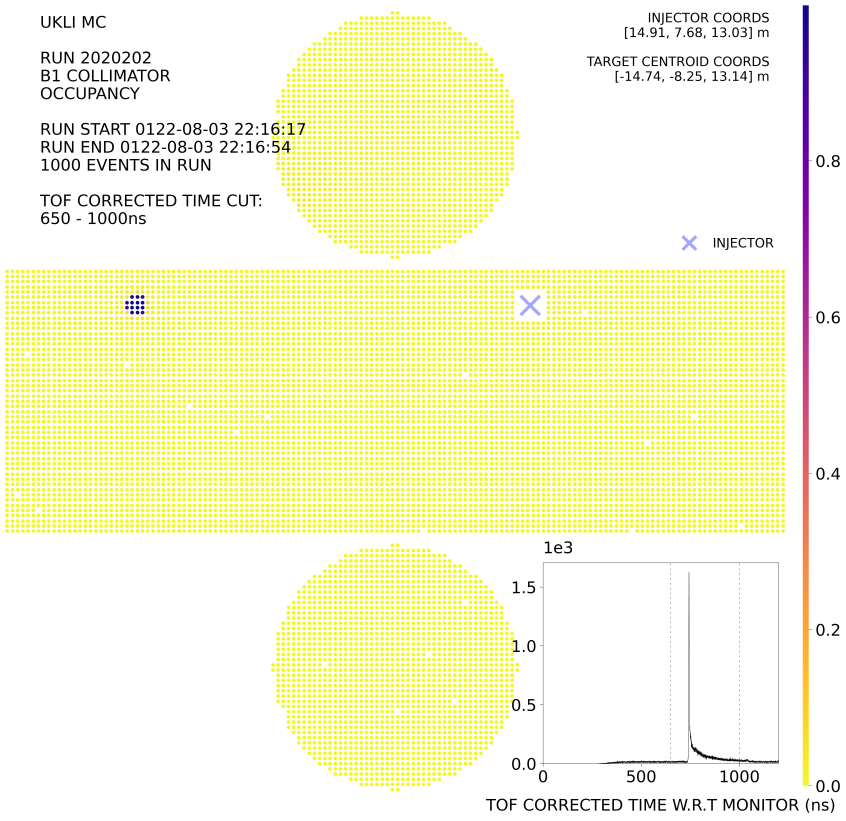
\includegraphics[width=0.9\textwidth]{Figures/ukli_mc_B1.PNG}
    \label{fig:ukli_mc_coll}
    \end{subfigure}\hfill
    \begin{subfigure}{0.49\columnwidth}
    \centering
    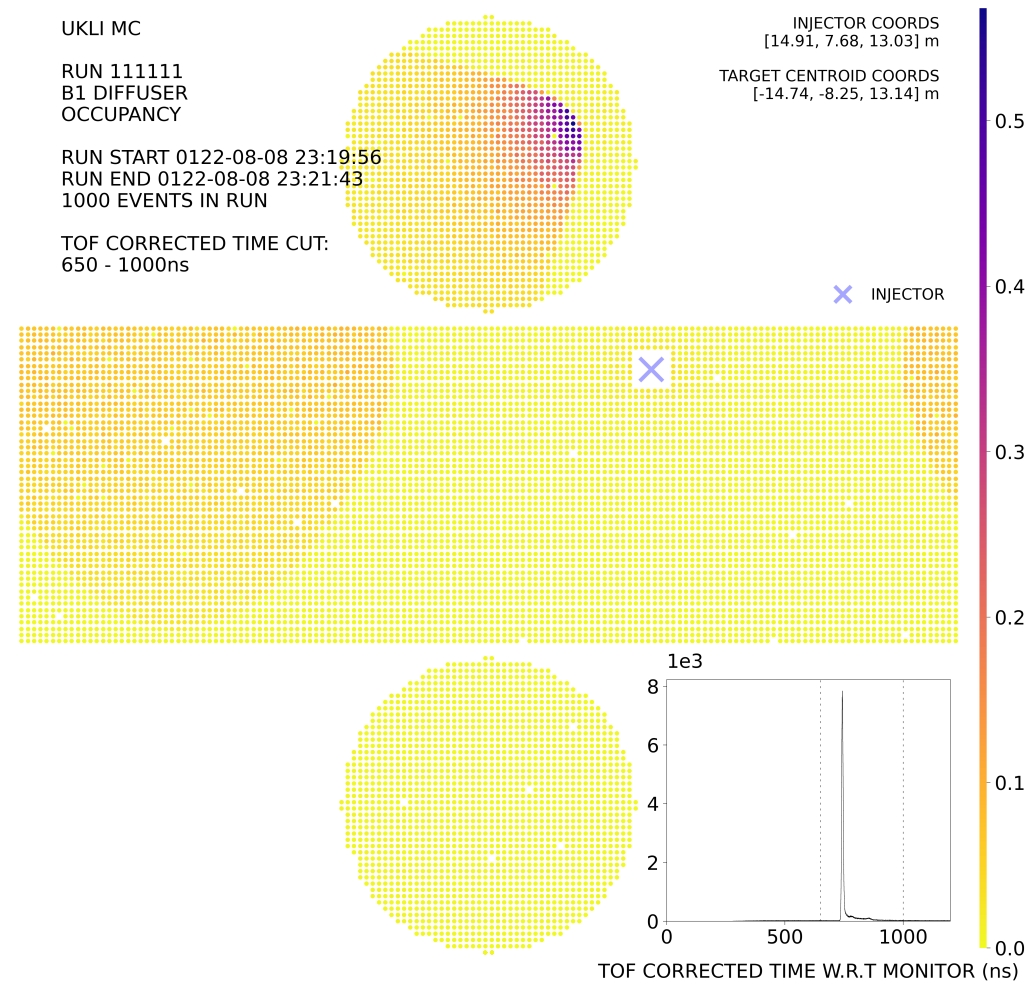
\includegraphics[width=0.9\textwidth]{Figures/ukli_diff_mc_B1.PNG}
    \label{fig:ukli_mc_diff}
    \end{subfigure}
    \caption{Monte Carlo simulations of the B1 collimator (left) and diffuser (right) injectors}
    \label{fig:ukli_mc_diff_coll}
\end{figure}

In order to validate the diffuser MC inverse cumulative distribution function output, a uniform distribution was run through the equation for the diffuser inverse CDF fits and the original PDF fit for each diffuser was used to fit the output points from the distribution, showing that inverse transform sampling was done correctly for the PDFs. This is shown for the B1 diffuser in Figure \ref{fig:inv_cdf_check}. 

\begin{figure}
    \centering
    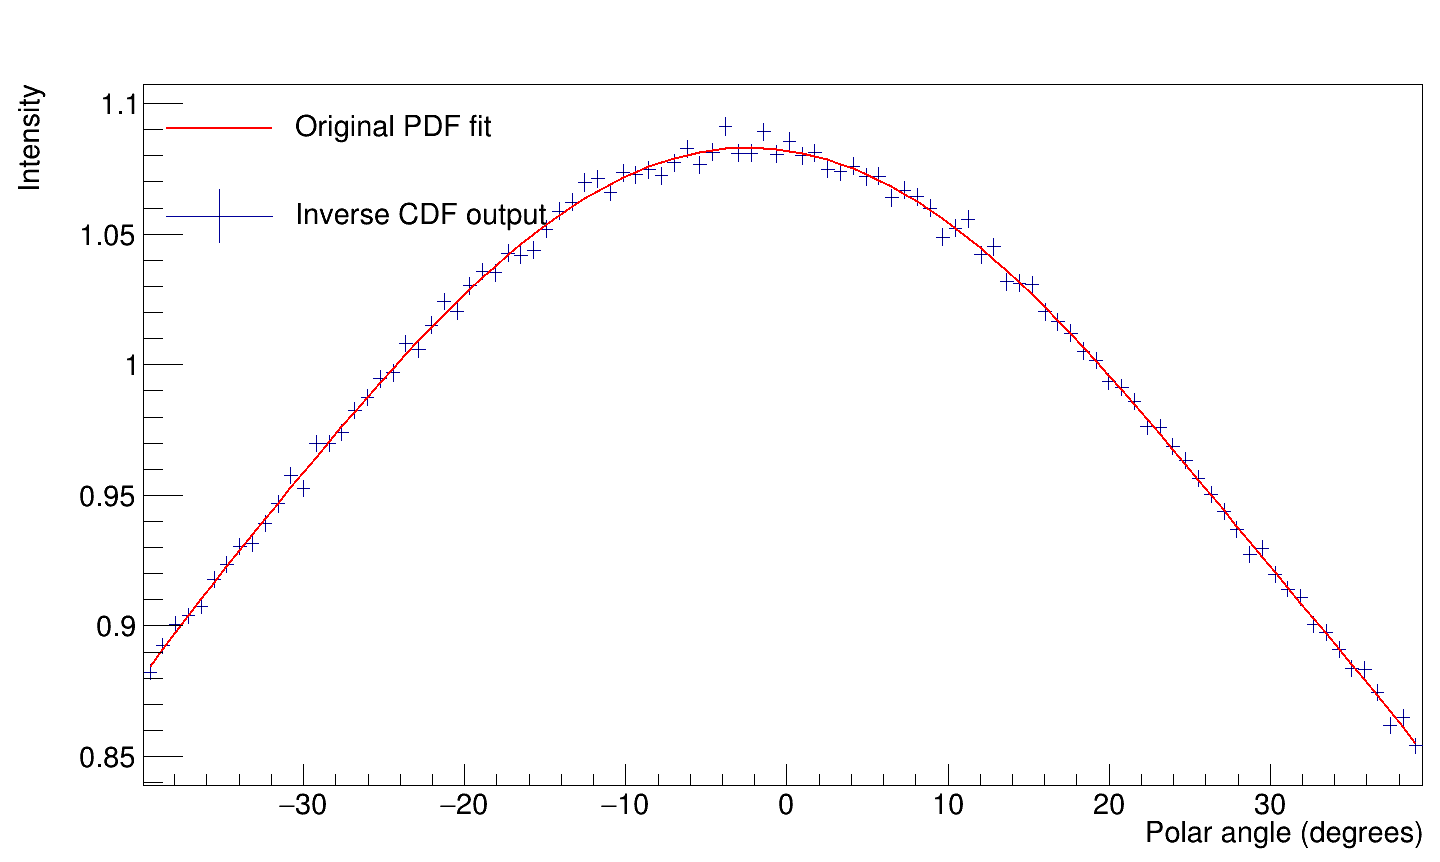
\includegraphics[width=0.9\textwidth]{Figures/inv_cdf_check_diff_B1.PNG}
    \caption{B1 diffuser inverse CDF check}
    \label{fig:inv_cdf_check}
\end{figure}


After producing the UKLI MC, adjusting the timing distributions in order to match up with the UKLI test run data was the next step. Producing time-of-flight corrected plots for the B1 collimator UKLI MC and overlaying it with the Run 82181 November test run data with the standard optical parameters, it was clear that there are disgreements between the Monte Carlo and data in both the scattered hits region and the reflected hits peak. In order to change this, the time dispersion of the injected photons in the MC was varied, in order to match the time dispersion of the injected photons in the data.

The time dispersion for the injected photons in the laser generation in SKDETSIM is governed by a Gaussian distributed random number generated using a Box-Muller transform, where additional time dispersion added would be the sigma of this Gaussian, and after a random number is passed through it, the output number would be added to the time for each track step of the photon giving the time dispersion.

The Box-Muller transform is a random number sampling method for making pairs of independent, normally distributed random sources from a source of uniformly distributed numbers (usually from between 0 and 1) \cite{10.1214/aoms/1177706645}. The form of the Box-Muller method implemented to calculate the added time dispersion is the Marsaglia polar method \cite{doi:10.1137/1006063}, which works by choosing two independent and uniformly distributed numbers (u,v) between [-1,+1], so that $s = u^{2} + v^{2}$, and if $s=0$, or $s>=1$, another pair of numbers are chosen. Then the standard normal deviate which is given by $$z_{0}=u \cdot \sqrt{\frac{-2 \ln s}{s}}$$ is multiplied by the chosen value of time dispersion in seconds and added to the mean (set to zero) to give the normally dispersed extra track step time for a photon in the distribution. 

Figure \ref{fig:gauss_time_dispersion} shows the effect of implementing this varying time dispersion on the raw hit timing output from the UKLI MC B1 collimator simulation, with the time dispersion shown for 0 ns, 5 ns, 10 ns, 15 ns and 20 ns. 

\begin{figure}
    \centering
    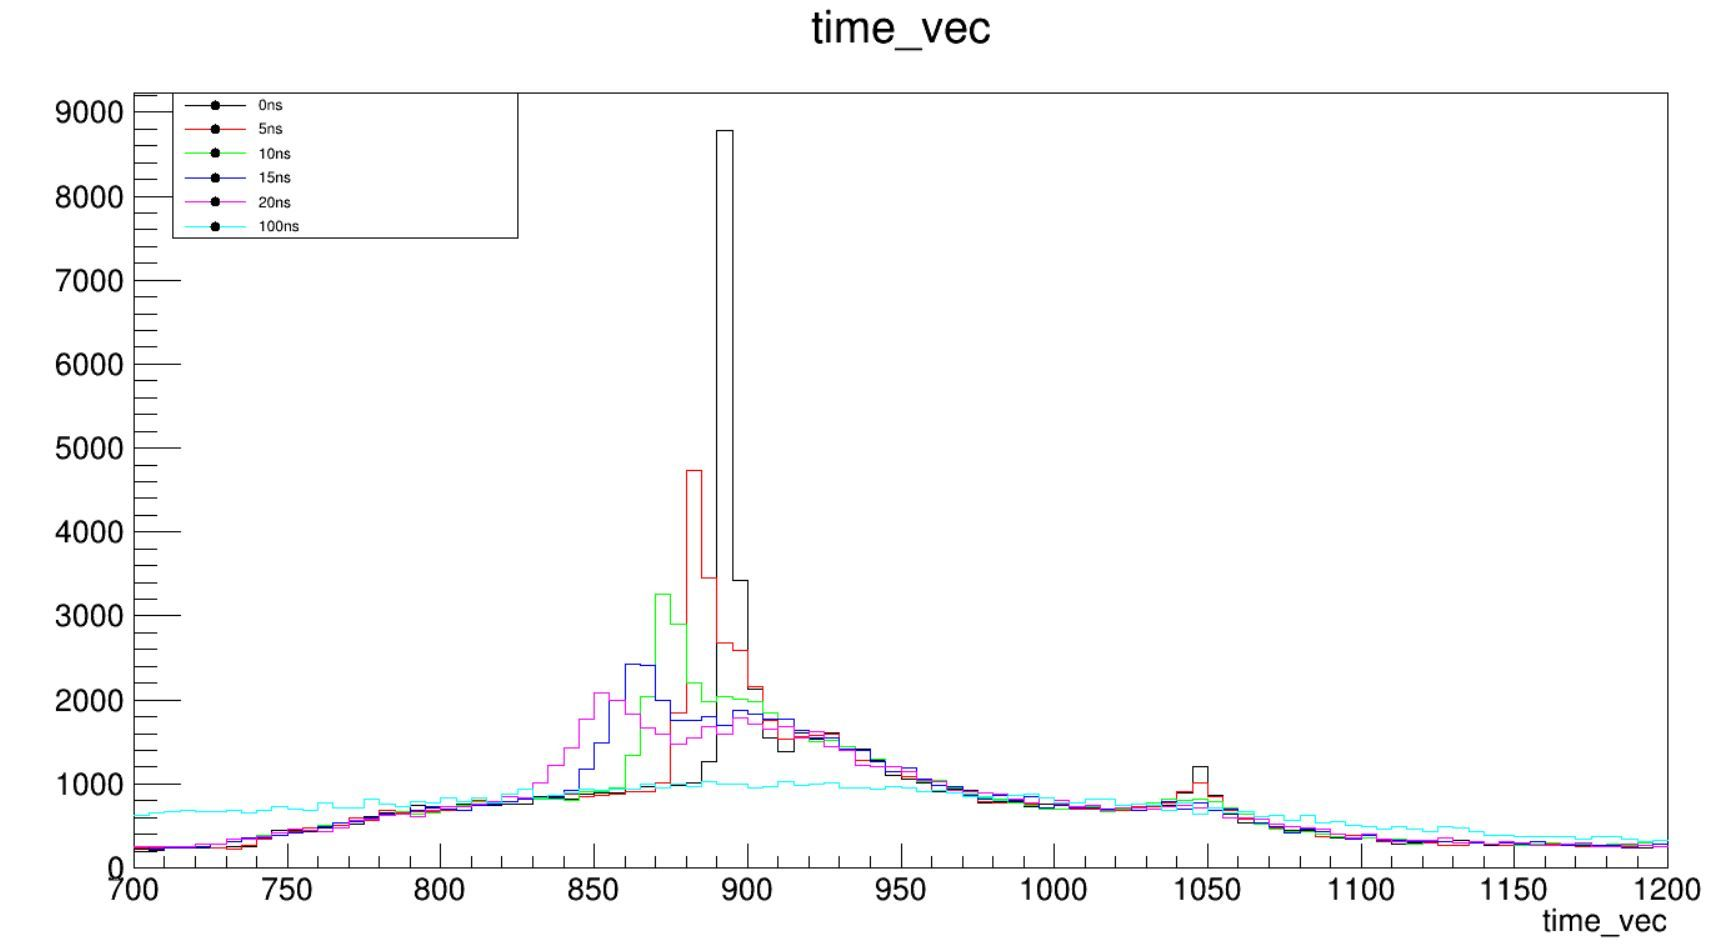
\includegraphics[width=\textwidth]{Figures/gauss_time_dispersion.PNG}
    \caption{Gaussian distributed time dispersion plots, with varying amounts of time dispersion}
    \label{fig:gauss_time_dispersion}
\end{figure}

In order to properly compare the timing distributions between data and Monte Carlo, the time-of-flight corrected timing plots are produced. To only select reflected and scattered hits, an exclusion region of hits is set: this is set to be $\pm$ 2 m around the injector (in order to avoid using backscattered hits in the analysis), and also $\pm$ 3.2 m around the injector target region in order to avoid including direct hits to the beam target. Figure \ref{fig:exclusion_region} shows the regions for the hits which are included and excluded in order to produce the TOF corrected timing distributions.

\begin{figure}
    \centering
    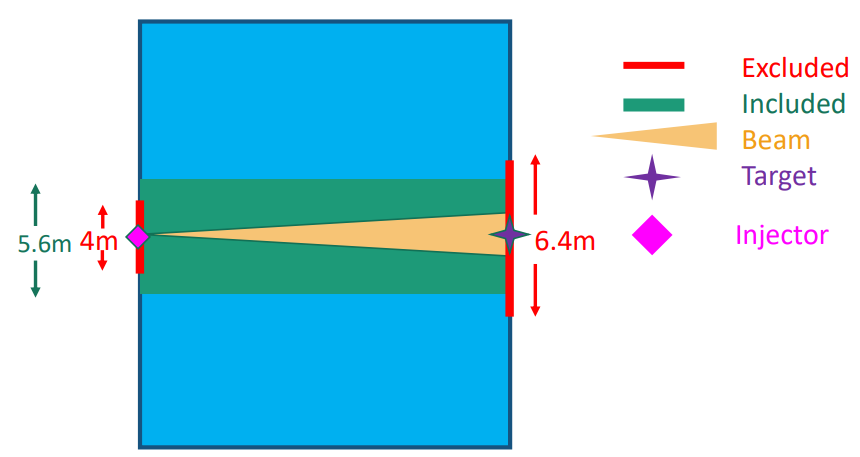
\includegraphics[width=\textwidth]{Figures/exclusion_region.PNG}
    \caption{The included (green) and excluded (red) regions for the TOF timing distributions}
    \label{fig:exclusion_region}
\end{figure}

Figures \ref{fig:0ns_time_dispersion}, \ref{fig:5ns_time_dispersion}, \ref{fig:10ns_time_dispersion}, \ref{fig:15ns_time_dispersion}, \ref{fig:20ns_time_dispersion} show time-of-flight corrected hit timing distributions for the B1 injector. The region between the blue dashed lines are the region for the scattered hits and the peak on the right shows the reflected hits. The hits from the injector data are shown in black and the MC hits are shown in red. In order to find the closest match for the time dispersion in the data, a gaussian distribution was fit to the B1 collimator data and Monte Carlo reflected peaks and the width of the gaussian was compared - this was only done for the 10 ns, 15 ns and 20 ns dispersion plots because the value for the time dispersion for the LED pulse is known to be in this range and the peak is too narrow and uneven for the 0 ns and 5 ns dispersion plots to fit a gaussian properly. The reason for the variation in the height of the reflected peaks between the MC and data is due to the detector response, which is why the width is being focussed on here instead.

\begin{figure}
    \centering
    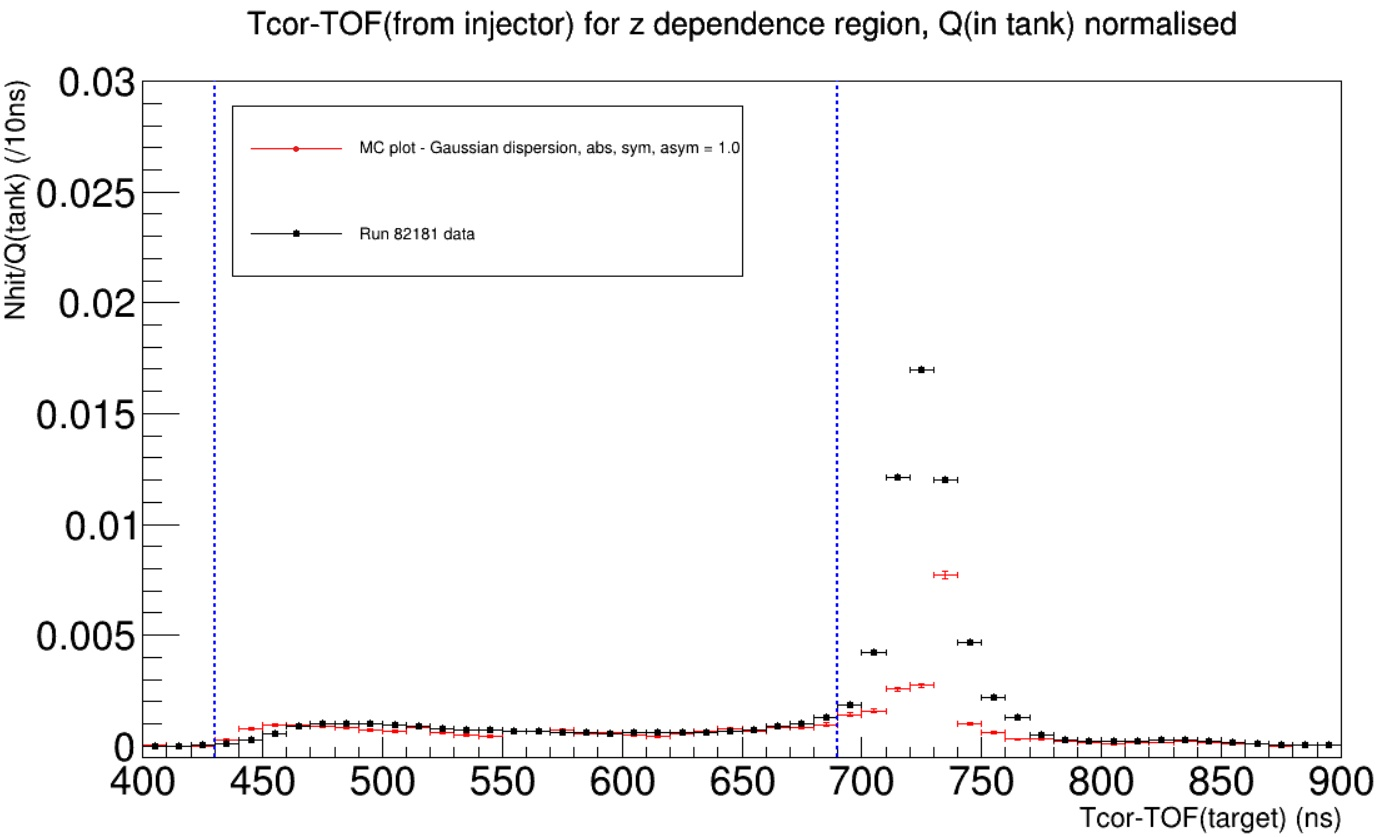
\includegraphics[width=\textwidth]{Figures/0ns_gaussian_dispersion_comparison.jpg}
    \caption{TOF comparison between UKLI MC with no time dispersion and Run 82181 test data for B1 collimator}
    \label{fig:0ns_time_dispersion}
\end{figure}

\begin{figure}
    \centering
    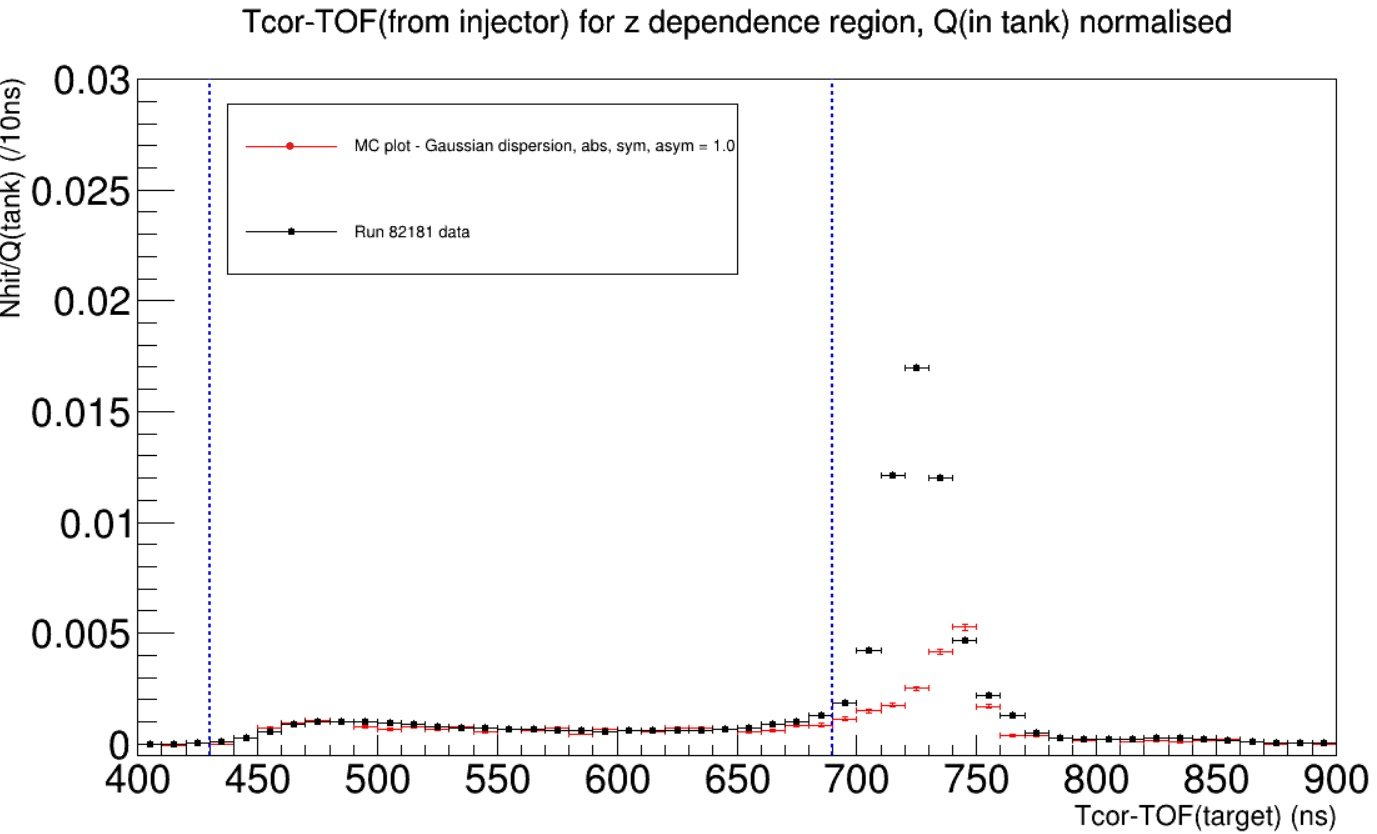
\includegraphics[width=\textwidth]{Figures/Inked5ns_gaussian_dispersion_comparison.jpg}
    \caption{TOF comparison between UKLI MC with 5 ns gaussian time dispersion and Run 82181 test data for B1 collimator}
    \label{fig:5ns_time_dispersion}
\end{figure}

\begin{figure}
    \centering
    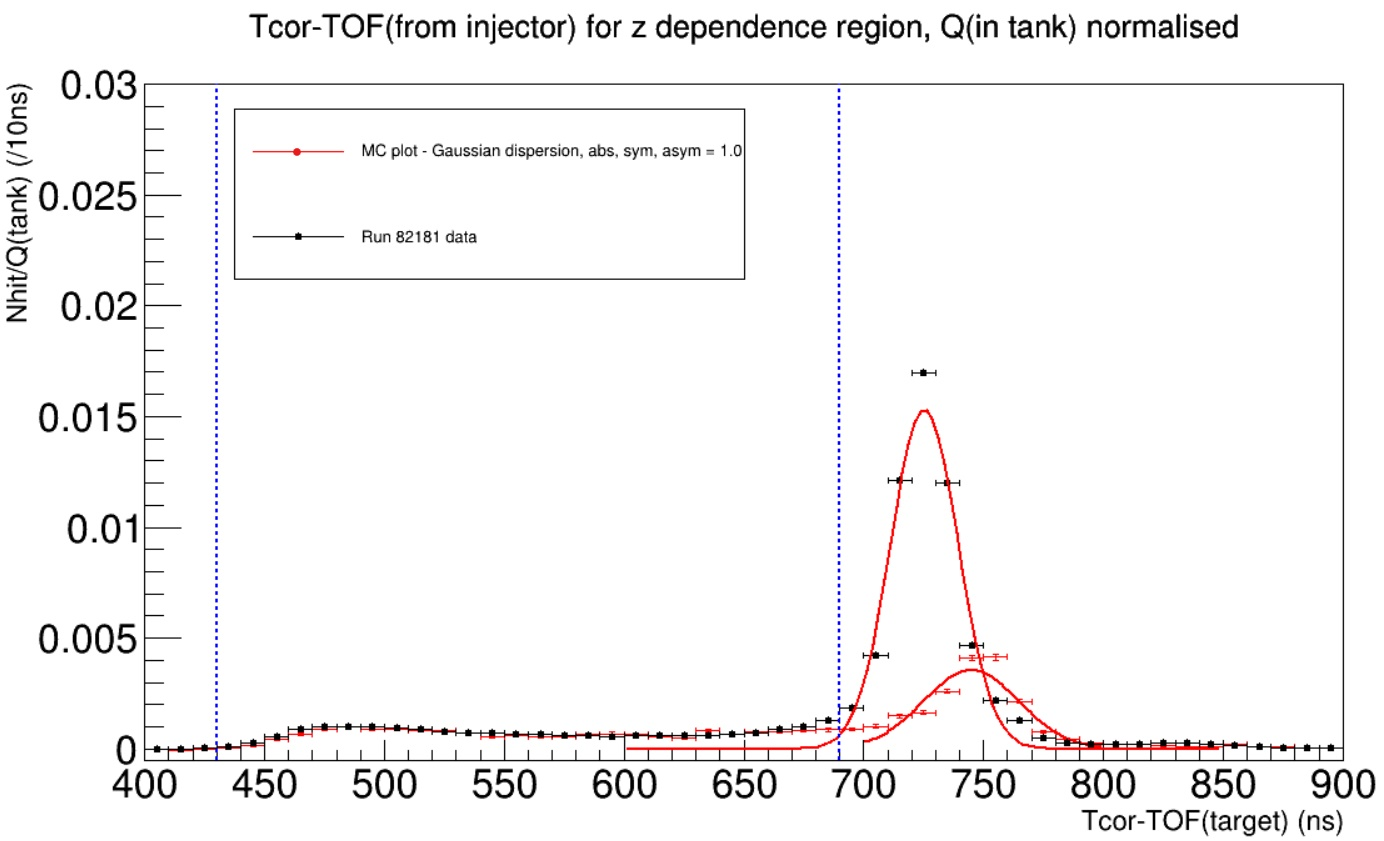
\includegraphics[width=\textwidth]{Figures/Inked10ns_gaussian_dispersion_with_fit.jpg}
    \caption{TOF comparison between UKLI MC with 10 ns gaussian time dispersion and Run 82181 test data for B1 collimator, with a gaussian fit to both}
    \label{fig:10ns_time_dispersion}
\end{figure}

\begin{figure}
    \centering
    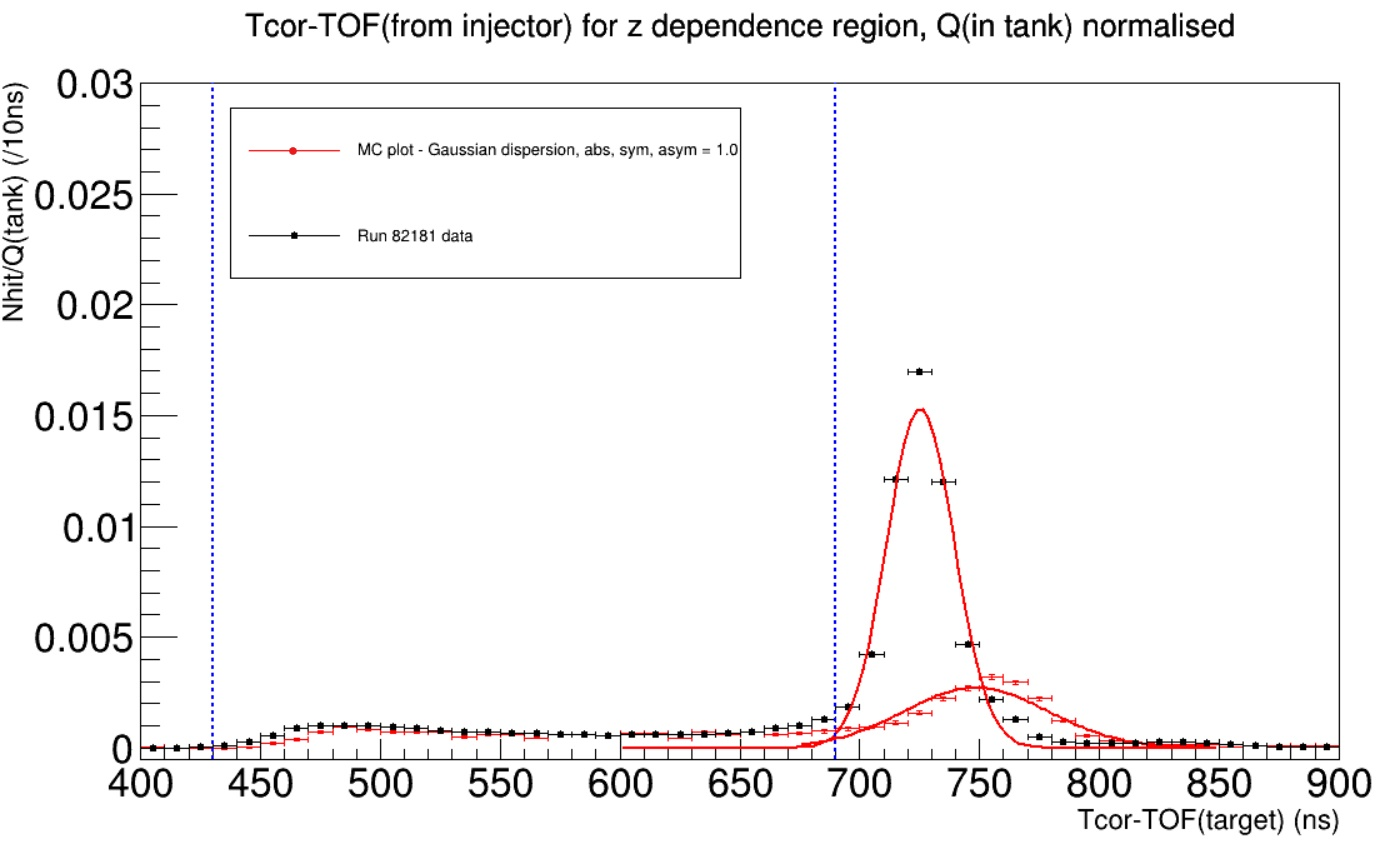
\includegraphics[width=\textwidth]{Figures/Inked15ns_gaussian_dispersion_with_fit.jpg}
    \caption{TOF comparison between UKLI MC with 15 ns gaussian time dispersion and Run 82181 test data for B1 collimator, with a gaussian fit to both}
    \label{fig:15ns_time_dispersion}
\end{figure}

\begin{figure}
    \centering
    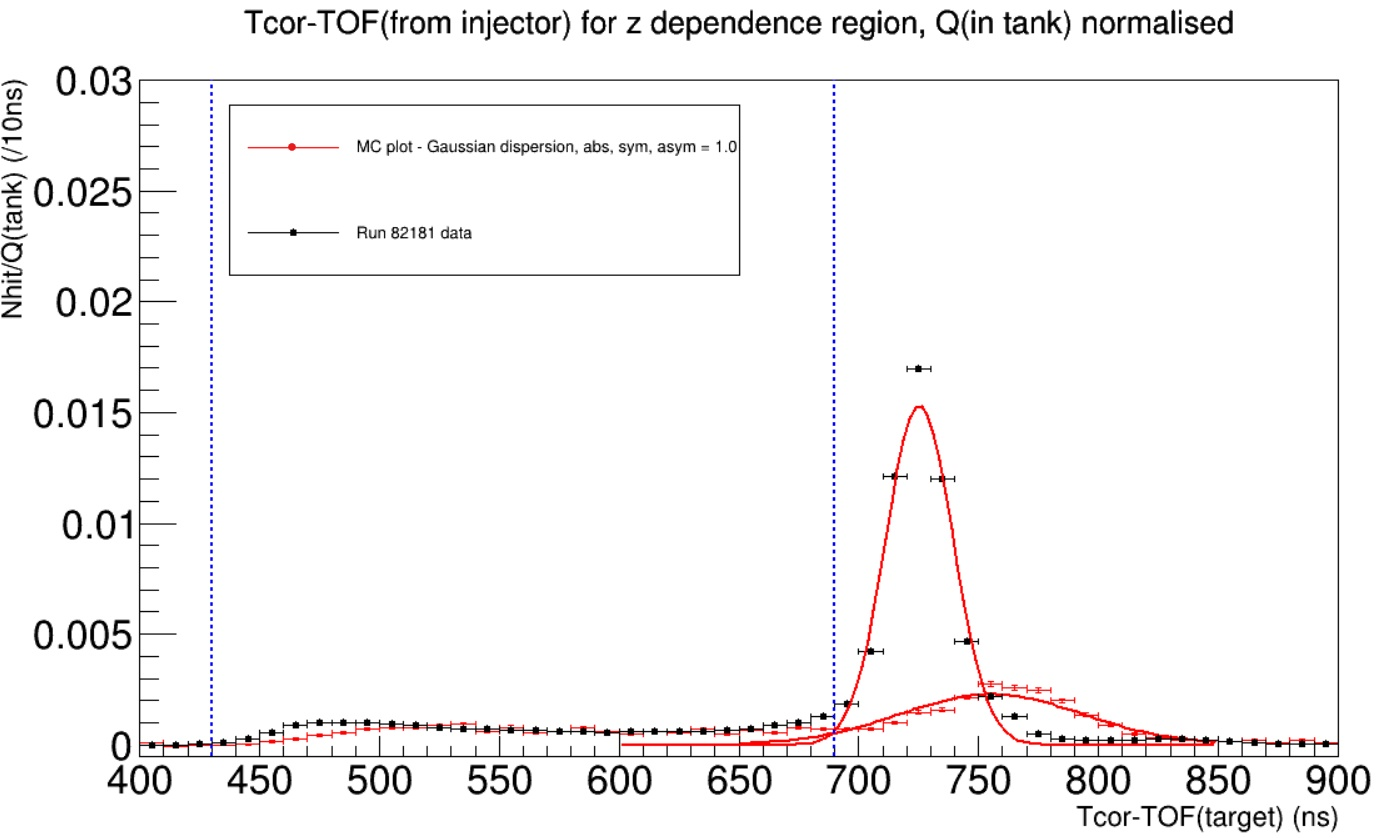
\includegraphics[width=\textwidth]{Figures/Inked20ns_gaussian_dispersion_with_fit.jpg}
    \caption{TOF comparison between UKLI MC with 20 ns gaussian time dispersion and Run 82181 test data for B1 collimator, with a gaussian fit to both}
    \label{fig:20ns_time_dispersion}
\end{figure}


The sigma of the gaussian fit to the data is 14.07 $\pm$ 0.01 ns, while the gaussian fit to the reflected peak for the 10 ns, 15 ns, and 20 ns time dispersed MC distributions is shown in Table \ref{table:reflected_peak_gaussian}. 

\begin{table}[htp]
\centering
\begin{tabular}{||c|c|c||}
     \hline Time dispersion value $(\mathrm{ns})$ & Sigma of gaussian $(\mathrm{ns})$ & $\chi^2 / n d f$ values of scattered hits region \\
    \hline 0 & - & 8.15 \\
    \hline 5 & - & 4.72 \\
    \hline 10 & $19.94 \pm 0.39$ & 3.45 \\
    \hline 15 & $30.30 \pm 0.55$ & 13.17 \\
    \hline 20 & $38.46 \pm 0.75$ & 22.12 \\
    \hline 
\end{tabular}   
\caption{Sigma of gaussian (ns) for each value of time dispersion along wth the $\chi^2/ndf$ value for B1 data and MC comparison between the scattered hits region (blue dashed lines).} 
\label{table:reflected_peak_gaussian}
\end{table}

From Table \ref{table:reflected_peak_gaussian} it can be seen that the 10 ns dispersion had the closest value to the B1 data for the sigma of the gaussian fit to the reflected peak, and also the lowest $\chi^2/ndf$ value (where the number of deegrees of freedom $ndf$ = 26) for the comparison between the data and MC for the scattered hits region, showing that this 10 ns dispersion was the best to use in the MC. In order to improve this part of the analysis, the scale of the time dispersion values could be more granular, for example, zooming into the 5 - 10 ns range when producing MC in order to more accurately determine the value of the time dispersion for the collimator data.

To summarise the work in this Chapter, data from test stands using the same optics used in the UKLI in Super-Kamiokande were used to produce probability and cumulative distribution functions of the optic light profiles. These were implemented into the Super-Kamiokande detector simulation, and inverse transform sampled in order to produce UKLI MC beam spot outputs which were fitted with the original PDFs to verify the output. Alongside this, in order to better align the hit timing distributions for the MC and data, modifying the track step of the photon in the simulation was used to vary the time dispersion of the hits from the injector. The width of the reflected hits peak in TOF corrected timing distributions was determined with a gaussian fit, and compared with the B1 collimator data, along with a comparison of the difference in hit times in the scattered hits region, which allowed us to determine the optimal value for time dispersion of injected hits was 10 ns.
